\batchmode
\makeatletter
\def\input@path{{/home/cooperw/RStudio/Ranadu/R4RAF/}}
\makeatother
\documentclass[12pt,english]{report}\usepackage[]{graphicx}\usepackage[]{color}
% maxwidth is the original width if it is less than linewidth
% otherwise use linewidth (to make sure the graphics do not exceed the margin)
\makeatletter
\def\maxwidth{ %
  \ifdim\Gin@nat@width>\linewidth
    \linewidth
  \else
    \Gin@nat@width
  \fi
}
\makeatother

\definecolor{fgcolor}{rgb}{0.345, 0.345, 0.345}
\newcommand{\hlnum}[1]{\textcolor[rgb]{0.686,0.059,0.569}{#1}}%
\newcommand{\hlstr}[1]{\textcolor[rgb]{0.192,0.494,0.8}{#1}}%
\newcommand{\hlcom}[1]{\textcolor[rgb]{0.678,0.584,0.686}{\textit{#1}}}%
\newcommand{\hlopt}[1]{\textcolor[rgb]{0,0,0}{#1}}%
\newcommand{\hlstd}[1]{\textcolor[rgb]{0.345,0.345,0.345}{#1}}%
\newcommand{\hlkwa}[1]{\textcolor[rgb]{0.161,0.373,0.58}{\textbf{#1}}}%
\newcommand{\hlkwb}[1]{\textcolor[rgb]{0.69,0.353,0.396}{#1}}%
\newcommand{\hlkwc}[1]{\textcolor[rgb]{0.333,0.667,0.333}{#1}}%
\newcommand{\hlkwd}[1]{\textcolor[rgb]{0.737,0.353,0.396}{\textbf{#1}}}%
\let\hlipl\hlkwb

\usepackage{framed}
\makeatletter
\newenvironment{kframe}{%
 \def\at@end@of@kframe{}%
 \ifinner\ifhmode%
  \def\at@end@of@kframe{\end{minipage}}%
  \begin{minipage}{\columnwidth}%
 \fi\fi%
 \def\FrameCommand##1{\hskip\@totalleftmargin \hskip-\fboxsep
 \colorbox{shadecolor}{##1}\hskip-\fboxsep
     % There is no \\@totalrightmargin, so:
     \hskip-\linewidth \hskip-\@totalleftmargin \hskip\columnwidth}%
 \MakeFramed {\advance\hsize-\width
   \@totalleftmargin\z@ \linewidth\hsize
   \@setminipage}}%
 {\par\unskip\endMakeFramed%
 \at@end@of@kframe}
\makeatother

\definecolor{shadecolor}{rgb}{.97, .97, .97}
\definecolor{messagecolor}{rgb}{0, 0, 0}
\definecolor{warningcolor}{rgb}{1, 0, 1}
\definecolor{errorcolor}{rgb}{1, 0, 0}
\newenvironment{knitrout}{}{} % an empty environment to be redefined in TeX

\usepackage{alltt}
\usepackage{mathptmx}
\usepackage[T1]{fontenc}
\usepackage[letterpaper]{geometry}
\geometry{verbose,tmargin=3.54cm,bmargin=2.54cm,lmargin=2.54cm,rmargin=2.54cm,headheight=1cm,headsep=2cm,footskip=0.5cm}
\usepackage{fancyhdr}
\pagestyle{fancy}
\setlength{\parskip}{\medskipamount}
\setlength{\parindent}{0pt}
\usepackage{babel}
\PassOptionsToPackage{normalem}{ulem}
\usepackage{ulem}
\usepackage[unicode=true]
 {hyperref}

\makeatletter
%%%%%%%%%%%%%%%%%%%%%%%%%%%%%% Textclass specific LaTeX commands.
\newenvironment{lyxlist}[1]
	{\begin{list}{}
		{\settowidth{\labelwidth}{#1}
		 \setlength{\leftmargin}{\labelwidth}
		 \addtolength{\leftmargin}{\labelsep}
		 \renewcommand{\makelabel}[1]{##1\hfil}}}
	{\end{list}}

%%%%%%%%%%%%%%%%%%%%%%%%%%%%%% User specified LaTeX commands.
% use this only for the .tex version used for latex2html:
\renewenvironment{kframe}{\vskip0.1in\hrule}{\hrule\vskip0.1in} 

\makeatother
\IfFileExists{upquote.sty}{\usepackage{upquote}}{}
\begin{document}
This note records some preliminary thoughts regarding a possible R-based
web site that documents R tools for use with the RAF-aircraft netCDF
files. The thought is that this might be either a static or a shinyApp
site providing guidance and access to Ranadu, modified to be more
consistent with the tools described in ``R for Data Science'' by
Wickham.



\chapter{Introduction}

The intent of this web site is to assist new users of NCAR/EOL/RAF-produced
aircraft data if they would like to use R in their data analysis projects.
The intent here is to provide ``layers'', starting with a very simple
guide to constructing preliminary plots and extending to more advanced
uses of R, RStudio, and knitr to produce manuscripts and reproducible
and documented data-analysis projects.The emphasis here is on ``Ranadu'',
an R package that is intended to facilitate use of the data archives
produced by the data systems on the NSF/NCAR/EOL/RAF research aircraft.
(NSF=National Science Foundation; NCAR=National Center for Atmospheric
Research; EOL=Earth Observing Laboratory; RAF=Research Aviation Facility)
All the recent data files are in netCDF format, so that is the format
emphasized here. Those files contain measurements made in field campaigns
that use the NSF research aircraft operated by NCAR, presently consisting
of a C-130 and a Gulfstream V. A list of recent projects is available
at \href{http://www.eol.ucar.edu/all-field-projects-and-deployments/}{this EOL web page},
and data requests can be made via links on that page. Information
regarding the instruments and the processing algorithms are available
at these respective web sites: \href{https://www.eol.ucar.edu/aircraft-instrumentation}{https://www.eol.ucar.edu/aircraft-instrumentation}
and \href{https://github.com/NCAR/aircraft_ProcessingAlgorithms/blob/master/ProcessingAlgorithms.pdf}{ProcessingAlgorithms.pdf}.
The latter also provides references to the netCDF format, the variable
names in common use, and algorithms used to calculate the variables
in the data files.

\chapter{Getting Started}

This chapter or ``layer'' summarizes a few key tools that will enable
a new user to get started. Of course, it is certainly possible to
work with the NCAR/EOL/RAF data files using R routines without reference
to the ``Ranadu'' package featured here, but this discussion will
describe use of that package. There are instructions for installing
the package in the ``RanaduManual.pdf'', and there it is also recommended
to use RStudio as the user GUI for working with R\@. Once R, RStudio
and Ranadu are installed, it will be simple to use the functions highlighted
in the remainder of this chapter to get started. The key functions
are getNetCDF(), for reading the netCDF file and producing an R data.frame
with the measurements, and DataFileInfo(), for checking the properties
of the netCDF file. These two functions provide a useful starting
point for all data-analysis projects.

\section{DataFileInfo()}

A useful first look at a netCDF file is provided by Ranadu::DataFileInfo(),
which returns characteristics like the project name, flight number,
date/times, variable names, and the data rate. In addition, this function
returns a set of ``measurands'' (measured properties of the atmosphere
like air temperature) and the set of variables that provide measurements
of that measurand. The measurands in a particular file (the one referenced
above) are shown below:

\begin{knitrout}
\definecolor{shadecolor}{rgb}{0.969, 0.969, 0.969}\color{fgcolor}\begin{kframe}
\begin{alltt}
\hlstd{Project} \hlkwb{<-} \hlstr{'WECAN'}
\hlstd{FlightNumber} \hlkwb{<-} \hlnum{6}
\hlstd{fname} \hlkwb{<-} \hlkwd{sprintf} \hlstd{(}\hlstr{'%s%s/%srf%02d.nc'}\hlstd{, Ranadu}\hlopt{::}\hlkwd{DataDirectory}\hlstd{(),}
         \hlstd{Project, Project, FlightNumber)}
\hlstd{FI} \hlkwb{<-} \hlkwd{DataFileInfo}\hlstd{(fname)}
\hlkwd{names} \hlstd{(FI}\hlopt{$}\hlstd{Measurands)}
\end{alltt}
\begin{verbatim}
##  [1] ""                                               
##  [2] "altitude"                                       
##  [3] "air_temperature"                                
##  [4] "air_pressure"                                   
##  [5] "atmosphere_number_content_of_aerosol_particles" 
##  [6] "dew_point_temperature"                          
##  [7] "water_vapor_pressure"                           
##  [8] "geopotential_height"                            
##  [9] "latitude"                                       
## [10] "longitude"                                      
## [11] "platform_speed_wrt_ground"                      
## [12] "height"                                         
## [13] "wind_from_direction"                            
## [14] "wind_speed"                                     
## [15] "humidity_mixing_ratio"                          
## [16] "barometric_altitude"                            
## [17] "platform_pitch_angle"                           
## [18] "atmosphere_cloud_liquid_water_content"          
## [19] "air_pressure_at_sea_level"                      
## [20] "effective_radius_of_cloud_liquid_water_particle"
## [21] "relative_humidity"                              
## [22] "platform_roll_angle"                            
## [23] "solar_azimuth_angle"                            
## [24] "solar_elevation_angle"                          
## [25] "solar_zenith_angle"                             
## [26] "platform_speed_wrt_air"                         
## [27] "platform_orientation"                           
## [28] "air_potential_temperature"                      
## [29] "equivelent_potential_temperature"               
## [30] "pseudo_equivalent_potential_temperature"        
## [31] "platform_course"                                
## [32] "virtual_temperature"                            
## [33] "eastward_wind"                                  
## [34] "northward_wind"                                 
## [35] "upward_air_velocity"
\end{verbatim}
\end{kframe}
\end{knitrout}

The variables that provide redundant measurements of a specific measurand
are named lists with the measurand name and can be displayed by printing
the measurand name, as in the following example:

\begin{knitrout}
\definecolor{shadecolor}{rgb}{0.969, 0.969, 0.969}\color{fgcolor}\begin{kframe}
\begin{alltt}
\hlstd{FI}\hlopt{$}\hlstd{Measurands}\hlopt{$}\hlstd{air_temperature}
\end{alltt}
\begin{verbatim}
## [1] "AT_A"    "AT_A2"   "AT_VXL2" "ATF1"    "ATH1"    "ATH2"    "ATX"
\end{verbatim}
\end{kframe}
\end{knitrout}

In addition, the ``long\_name'' describing a variable (e.g., here
``ATX'') can be found as follows:

\begin{knitrout}
\definecolor{shadecolor}{rgb}{0.969, 0.969, 0.969}\color{fgcolor}\begin{kframe}
\begin{alltt}
\hlstd{FI}\hlopt{$}\hlstd{LongNames[}\hlkwd{which}\hlstd{(}\hlstr{'ATX'} \hlopt{==} \hlstd{FI}\hlopt{$}\hlstd{Variables)]}
\end{alltt}
\begin{verbatim}
## [1] "Ambient Temperature, Reference"
\end{verbatim}
\end{kframe}
\end{knitrout}

To see all the lists of information contained in the DataFileInfo
list, print the names as follows:

\begin{knitrout}
\definecolor{shadecolor}{rgb}{0.969, 0.969, 0.969}\color{fgcolor}\begin{kframe}
\begin{alltt}
\hlkwd{names}\hlstd{(FI)}
\end{alltt}
\begin{verbatim}
##  [1] "Number"     "Project"    "Platform"   "DataFile"   "Start"     
##  [6] "End"        "Rate"       "LatMin"     "LatMax"     "LonMin"    
## [11] "LonMax"     "Variables"  "LongNames"  "Measurands"
\end{verbatim}
\end{kframe}
\end{knitrout}

Examining these can help a user understand what is included in a particular
data file.

\section{getNetCDF() and the resulting data.frame}

A central component of the Ranadu structure is the Ranadu data.frame,
produced by reading the netCDF data file. It has a structure similar
to that of a spreadsheet, with rows corresponding to measurement times
and columns corresponding to measurements. The data.frame has these
features:
\begin{enumerate}
\item Each row corresponds to a unique time, and times are sequential (possibly
with gaps). For data rates higher than 1~Hz, rows are produced for
each sample time; i.e., 25 rows per second for 25-Hz files. When variables
are present in the netCDF file at a slower rate, interpolation is
used to produce the higher rate.
\item Each measurement corresponds to a single column. When there are multiple
measurements of a given measurand (e.g., temperature), each individual
measurement has its own column. There is a significant exception:
For instruments producing size-distribution arrays, the entire array
occupies one column of the data.frame. 
\item Attributes describing the data.frame and the variables are carried
with the data.frame. For example, variables often have ``short\_name''
and ``long\_name'' attributes, and these can be examined by looking
at the variable attributes. Those attributes include one named ``label''
that is used by default to label plots.
\end{enumerate}
The data.frame is constructed by Ranadu::getNetCDF(fname, variables),
which uses the ncdf4 package of routines to read the netCDF file.
An example of a subset of the data.frame is shown here:

\newpage{}

\begin{knitrout}
\definecolor{shadecolor}{rgb}{0.969, 0.969, 0.969}\color{fgcolor}\begin{kframe}
\begin{alltt}
\hlstd{Project} \hlkwb{<-} \hlstr{'WECAN'}
\hlstd{FlightNumber} \hlkwb{<-} \hlnum{6}
\hlstd{fname} \hlkwb{<-} \hlkwd{sprintf} \hlstd{(}\hlstr{'%s%s/%srf%02d.nc'}\hlstd{, Ranadu}\hlopt{::}\hlkwd{DataDirectory}\hlstd{(),}
         \hlstd{Project, Project, FlightNumber)}
\hlstd{Variables} \hlkwb{<-} \hlstd{Ranadu}\hlopt{::}\hlkwd{standardVariables}\hlstd{(}\hlkwd{c}\hlstd{(}\hlstr{'UXC'}\hlstd{,} \hlstr{'VYC'}\hlstd{))}
\hlstd{Data} \hlkwb{<-} \hlstd{Ranadu}\hlopt{::}\hlkwd{getNetCDF}\hlstd{(fname, Variables)}
\hlkwd{print} \hlstd{(}\hlkwd{sprintf} \hlstd{(}\hlstr{'Data from data file %s'}\hlstd{, fname))}
\end{alltt}
\begin{verbatim}
## [1] "Data from data file /Data/WECAN/WECANrf06.nc"
\end{verbatim}
\begin{alltt}
\hlkwd{print} \hlstd{(tibble}\hlopt{::}\hlkwd{as_tibble}\hlstd{(Data))}  \hlcom{# or print(head(Data))}
\end{alltt}
\begin{verbatim}
## # A tibble: 23,191 x 18
##    Time                  ATX  DPXC   EWX GGALT  LATC  LONC MACHX    MR
##    <dttm>              <dbl> <dbl> <dbl> <dbl> <dbl> <dbl> <dbl> <dbl>
##  1 2018-08-03 20:00:30  26.7    NA    NA  874.  43.6 -116. 0.109    NA
##  2 2018-08-03 20:00:31  26.6    NA    NA  874.  43.6 -116. 0.113    NA
##  3 2018-08-03 20:00:32  26.9    NA    NA  874.  43.6 -116. 0.118    NA
##  4 2018-08-03 20:00:33  27.2    NA    NA  874.  43.6 -116. 0.126    NA
##  5 2018-08-03 20:00:34  27.2    NA    NA  874.  43.6 -116. 0.129    NA
##  6 2018-08-03 20:00:35  27.3    NA    NA  874.  43.6 -116. 0.135    NA
##  7 2018-08-03 20:00:36  27.1    NA    NA  874.  43.6 -116. 0.142    NA
##  8 2018-08-03 20:00:37  27.2    NA    NA  874.  43.6 -116. 0.145    NA
##  9 2018-08-03 20:00:38  27.3    NA    NA  874.  43.6 -116. 0.149    NA
## 10 2018-08-03 20:00:39  27.4    NA    NA  873.  43.6 -116. 0.152    NA
## # ... with 23,181 more rows, and 9 more variables: PALT <dbl>, PSXC <dbl>,
## #   QCXC <dbl>, TASX <dbl>, WDC <dbl>, WSC <dbl>, WIC <dbl>, UXC <dbl>,
## #   VYC <dbl>
\end{verbatim}
\end{kframe}
\end{knitrout}

Here is an explanation of some aspects of loading this data.frame:
\begin{enumerate}
\item Ranadu::DataDirectory() returns the location of the data directory
on various systems, to avoid the necessity of changing this when moving
among systems. It may return '/scr/raf\_data/' or '/Data/' or '\textasciitilde /Data/'
or the directory corresponding to the environment variable ``DATA\_DIR''
(as assigned on EOL computers), depending on the file system.
\item The function Ranadu::standardVariables() returns a set of commonly
used variable names. Additional variables provided to the routine
(here, 'UXC' and 'VYC') are added to the variable list.
\item Ranadu::getNetCDF() produces the data.frame. The special case where
Variables <- ``ALL'' will return all available variables.\footnote{But use this cautiously because size-distribution variables are special
and sometimes cause problems when manipulating the resulting data.frame.
This is discussed later in association with ``tibbles.''} Two additional optional arguments to getNetCDF() are ``Start''
and ``End''; if set, the range of time values in the data.frame
will be restricted to be between those two times. See ``?Ranadu::getNetCDF''
for complete information on this function.
\item The last statement, where the data.frame is converted to a tibble,
is used here because the print function for tibbles produces a more
concise and clearer format than that for a data.frame. ``print (head
(Data))'' could have been used also. More information on tibbles
is included later in this document. The resulting data.frame has 23,701
rows and 18 columns.
\end{enumerate}

\section{Using the data.frame}

\subsection{Simple Plots}

It is straightforward to plot variables in the data.frame using standard
R functions. For example, the following code plots the altitude vs.~time
using the data.frame loaded previously:

\begin{knitrout}
\definecolor{shadecolor}{rgb}{0.969, 0.969, 0.969}\color{fgcolor}\begin{kframe}
\begin{alltt}
\hlkwd{plot}\hlstd{(Data}\hlopt{$}\hlstd{Time, Data}\hlopt{$}\hlstd{GGALT,} \hlkwc{type}\hlstd{=}\hlstr{'l'}\hlstd{)}
\end{alltt}
\end{kframe}\begin{figure}

{\centering 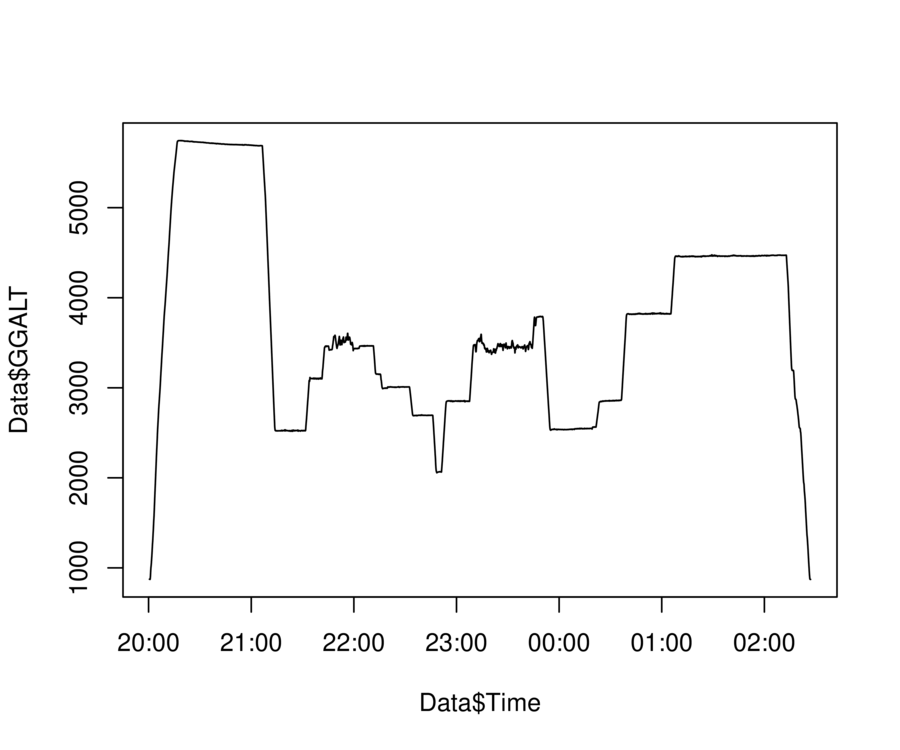
\includegraphics[width=\maxwidth]{figure/simple-plot1-1} 

}

\caption[Geometric altitude vs time for WECAN research flight 6, 3 August 2018]{Geometric altitude vs time for WECAN research flight 6, 3 August 2018.}\label{fig:simple-plot1}
\end{figure}


\end{knitrout}

Many of the Ranadu tools are aimed at making construction of such
plots straightforward while supporting various manipulations of the
style and content of the plots. Many of these are discussed in later
chapters. However, at this point you will be able to conduct extensive
data-analysis projects using only the standard tools provided by R.

\pagebreak{}

\subsection{Using plotWAC() and ggplotWAC()}

The function Ranadu::plotWAC() calls the standard R function ``plot''
with a particular set of conventions. Some reasons you may want to
consider using it include the following:
\begin{lyxlist}{00.00.0000}
\item [{time~offset:}] The convention in the NCAR/EOL/RAF netCDF files
is that the time variable represents the start of the interval over
which measurements are averaged, so a 1-Hz variable with a specified
time is actually an average where the mean time is 0.5~s later. Plots
generated by plotWAC() adjust for this offset. For this same reason,
you may want to use the routine Ranadu::lineWAC() to add lines to
the plot, instead of the standard ``lines'' routine provided by
R.
\item [{plot~format:}] The set of conventions regarding time labels, axis
formats, and legends may be preferable to those that are standard
with ``plot()'' and will save you from making those tailoring adjustments.
\item [{pipe\_compatible:}] The function plotWAC() can be used in a pipe
where the piped variable is a data.frame tailored to contain specified
variables to construct multiple-variable plots. A similar pipe to
``plot()'' will produce a faceted plot of each variable vs.~each
other variable, which may not be what you want.
\end{lyxlist}
Figure \ref{fig:plotwac-ex} shows an example.

\begin{knitrout}
\definecolor{shadecolor}{rgb}{0.969, 0.969, 0.969}\color{fgcolor}\begin{kframe}
\begin{alltt}
\hlkwd{plotWAC}\hlstd{(Data[,} \hlkwd{c}\hlstd{(}\hlstr{'Time'}\hlstd{,} \hlstr{'GGALT'}\hlstd{)])}
\end{alltt}
\end{kframe}\begin{figure}

{\centering 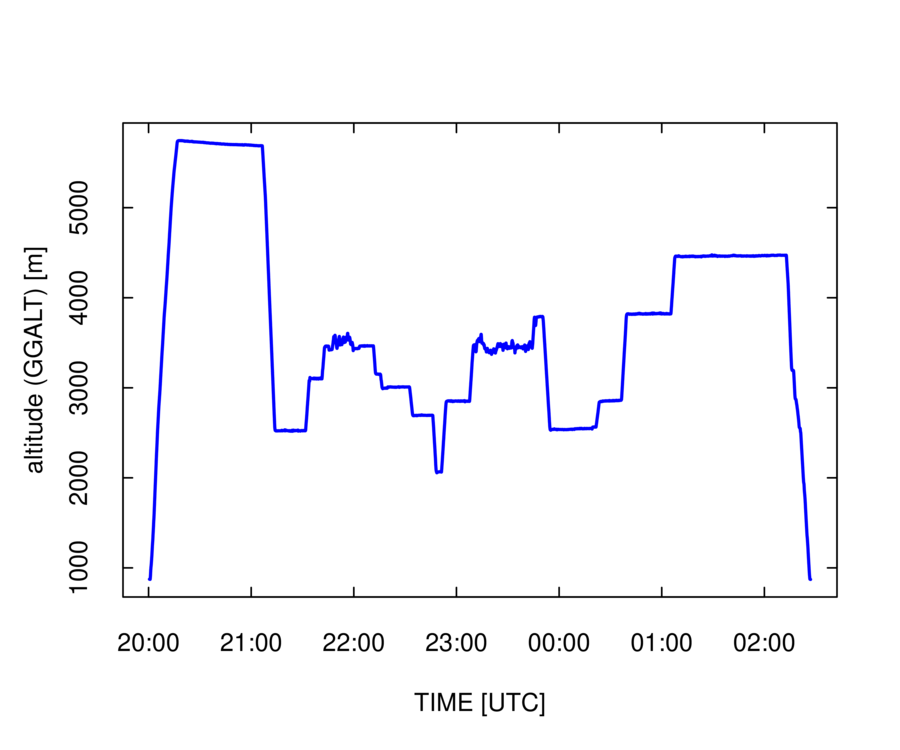
\includegraphics[width=\maxwidth]{figure/plotwac-ex-1} 

}

\caption[Example of the same plot as the preceding figure but generated with Ranadu::plotWAC()]{Example of the same plot as the preceding figure but generated with Ranadu::plotWAC().}\label{fig:plotwac-ex}
\end{figure}


\end{knitrout}

Another option is provided by Ranadu::ggplotWAC(), as shown in Fig.~\ref{fig:ggplot-ex}:

\begin{knitrout}
\definecolor{shadecolor}{rgb}{0.969, 0.969, 0.969}\color{fgcolor}\begin{kframe}
\begin{alltt}
\hlkwd{ggplotWAC}\hlstd{(Data[,} \hlkwd{c}\hlstd{(}\hlstr{'Time'}\hlstd{,} \hlstr{'GGALT'}\hlstd{)])}
\end{alltt}
\end{kframe}\begin{figure}

{\centering 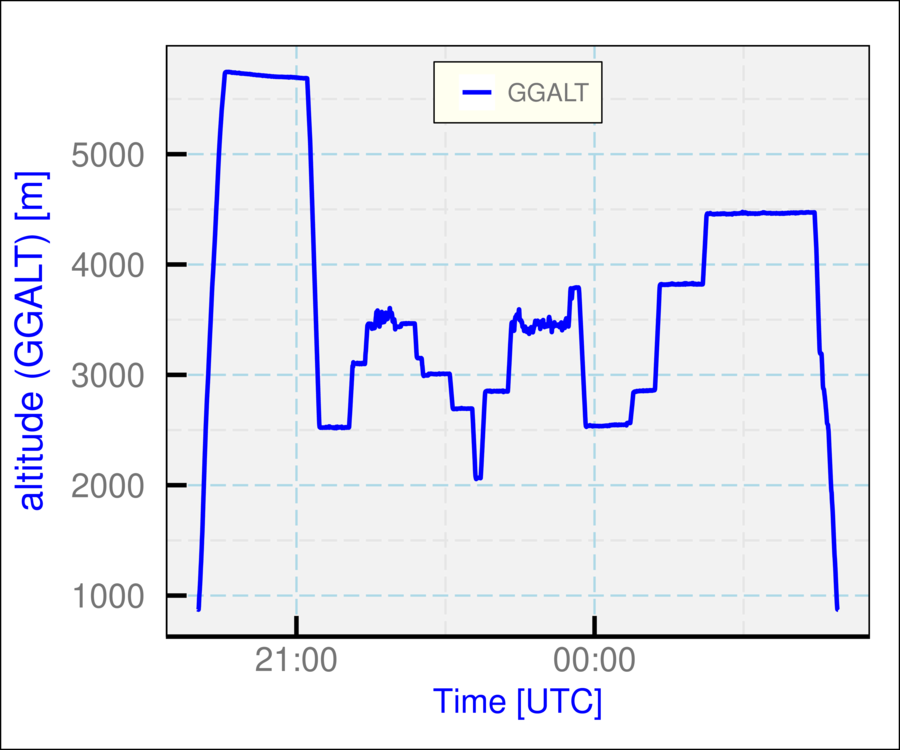
\includegraphics[width=\maxwidth]{figure/ggplot-ex-1} 

}

\caption[Example of the same plot as the preceding figure but generated with Ranadu::ggplotWAC()]{Example of the same plot as the preceding figure but generated with Ranadu::ggplotWAC().}\label{fig:ggplot-ex}
\end{figure}


\end{knitrout}

Additional examples showing the advantages of constructing plots with
pipes will be presented in later chapters of this document. For more
information on the use of these plotting routines, see ``?Ranadu::plotWAC''
and ``?Ranadu::ggplotWAC''.

\pagebreak{}

\chapter{Overview of Ranadu functions}

A more extensive discussion if Ranadu is contained in the Ranadu Manual,
available here\href{https://github.com/NCAR/Ranadu/blob/WAC/inst/RanaduManual.pdf}{here}.
Some of the central features are discussed in this chapter.

\section{More about constructing data.frames}

These Ranadu functions can be of use when constructing and modifying
data.frames:
\begin{itemize}
\item \texttt{getNetCDF ( )}: loads a data.frame with requested variables
\item \texttt{standardVariables( ):} defines a common set of variables for
input to getNetCDF(). This list is the default if no variables are
specified in the call to getNetCDF. The optional argument is a list
of character names that specify additional variables to include.
\item \texttt{DataDirectory( ): }This is system dependent and is intended
to aid in portability by providing the usual location of the netCDF
data files. It tries a set of likely names, but may need redefinition
for some file systems.
\item \texttt{getProjectData( ):} Constructs a data.frame that includes
measurements from multiple flights in a project.
\item \texttt{getIndex( )}: finds the index for a specified time
\item \texttt{setRange( )}: sets a range of indices covering a specified
time interval.
\item \texttt{selectTimes( ):} produces a new data.frame with a limited
time range.
\end{itemize}
In addition, some functions provided by the package ``dplyr'' can
be very useful when working with data.frames. These actions can be
implemented by normal R subsetting also (e.g., using ``{[}{[}...{]}{]}''
notation), but using these dplyr functions serves to clarify what
the steps in the code are doing:
\begin{itemize}
\item \texttt{dplyr::select( ):} produces a new data.frame with only the
variables listed as arguments in the call to the function.
\item \texttt{dplyr::filter( ):} produces a subset data.frame where the
argument is a logical test applied to the data.frame rows that must
be met for the row to be included in the returned data.frame.
\item \texttt{dplyr::mutate( ):} adds new variables to the data.frame. \texttt{Ranadu::Rmutate(
)} modifies this to preserve variable attributes.
\end{itemize}
The related function Ranadu::selectTime( ) can be used to restrict
the times included in the data.frame, so it is often convenient to
use this routine in combination with the above routines when constructing
plots and for other data-analysis steps. See akso \texttt{Ranadu::RSubset(
).}

\section{Getting information about the data}

Many Ranadu functions provide information about the data set. A good
starting point is DataFileInfo(), discussed in the previous chapter.
In addition, these functions may be helpful:
\begin{enumerate}
\item \texttt{\uline{Ranadu::getAttributes():}} The data.frames produced
by getNetCDF() have assigned attributes that match those in the original
netCDF file, and these can be retrieved via getAttributes(), where
the argument can be either the data.frame (for which the returned
attributes are those associated with the data file) or a variable
name (for which the attributes are those associated with the variable).\footnote{Subsetting will often lose some attributes so special steps are needed
to preserve them if that is desired.} The result of the function call is a printed listing of attributes
and creation of a list (here in Z) that contains the attributes, so
it is usually preferable to assign the returned value to something
to avoid the double listing that would be produced otherwise.
\item \texttt{\uline{Ranadu::TellAbout()}} provides some information
about the characteristics of a data.frame or a variable in the data.frame.
\item \texttt{\uline{Ranadu::getStartEnd()}}\texttt{ }returns the start
and end times of a data frame.
\item \texttt{\uline{Ranadu::ValueOf() and Ranadu::ValueOfAll()}}\texttt{
}for a specified time return the value of a specified variable or
of all variables, respectively.
\end{enumerate}
The standard R routines ``dim()'', ``names()'' and ``str()''
will also provide information about a data.frame or a variable. ``str()''
in particular can provide important information about all R variables.

\section{Plotting routines}

The routines plotWAC() and ggplotWAC() were introduced in the previous
chapter. The following is a list of other Ranadu routines that produce
plots. More detail about these routines is included in the next chapter.
\begin{enumerate}
\item \texttt{\uline{Ranadu::plotTrack()}} plots a flight track on a
background that shows geographic boundaries. In its simplest form
it is called with a single argument of a data.frame that contains
at least latitude and longitude in variables named LATC and LONC.
This routine also has an option to plot the track in a reference frame
that drifts with the wind. See ?plotTrack for more information on
options.
\item \texttt{\uline{Ranadu::VSpec()}} constructs a plot of the variance
spectrum for a specified variable. See also \texttt{\uline{Ranadu::CohPhase()}}\texttt{
}for plots of the coherence and phase relationship between variables,
and \texttt{\uline{Ranadu::flux( )}} for plotting the cospectrum
and calculating various fluxes.
\item \texttt{\uline{Ranadu::lineWAC()}} adds a line to a plot previously
constructed by plotWAC(), with adjustment of the plotted time to correspond
to the center of the interval averaged to obtain the measurements.
Otherwise, like ``lines()'' in standard R.
\item \texttt{\uline{Ranadu::plotSD()}} plots the size distribution measured
by cloud or aerosol particle probes.
\item \texttt{\uline{Ranadu::contourPlot()}} plots a scattergram-like
display where the density of points is represented by colored areas.
This can be a useful alternative to a scatterplot when the number
of plotted points is large.
\item \texttt{\uline{Ranadu::DemingFit()}} calculates a Deming fit to
two variables (in which the distance from the fitted line to the two-dimensional
locations of the measurements is minimized) and plots the resulting
fit.
\item \texttt{\uline{Ranadu::SkewTSounding()}} plots a skew-T thermodynamic
diagram with measurements from a data.frame averaged and superimposed
on the diagram. Options are available to include a hodograph and the
denote values of the LCL and CAPE.
\end{enumerate}

\section{Computational Algorithms}

A set of functions provide calculations like those used to process
the original files and, in some cases, to extend those calculations.
A full list of Ranadu functions can be viewed by using the R command
``?Ranadu'', and clicking on the items in that list then will provide
the standard ``help'' information for the functions. Some of these
are listed below. For additional details, see the technical note titled
``Processing Algorithms''.
\begin{enumerate}
\item \texttt{AdiabaticTandLWC( ):} Calculate the temperature and liquid
water content produced by adiabatic ascent.
\item \texttt{AirTemperature( ):} The standard calculation of temperature
from the measured recovery temperature.
\item \texttt{BoltonEquivalentPotentialTemperature( ):} Equivalent potential
temperature as calculated using the Bolton formula. In standard processing,
this has been replaced now by the Davies-Jones representation; see
``EquivalentPotentialTemperature( )'' below.
\item \texttt{ButterworthFilter( ):} Implementation of a Butterworth low-pass
filter, used in wind processing; see ``ComplementaryFilter( )''.
\item \texttt{calcAttack( ):} This function calculates the angle of attack
from the pitch and rate of climb of the aircraft under the assumption
that the vertical wind is zero. This algorithm may be useful when
determining or checking sensitivity coefficients for the measured
angle of attack.
\item \texttt{ComplementaryFilter( ):} The standard calculation of wind
uses this complementary filter to combine the aircraft ground-speed
components measured by the inertial system at high rate with the corresponding
components measured by the global positioning system at lower rate.
\item \texttt{CorrectHeading( ), CorrectPitch( ) }and\texttt{ CorrectRoll(
): }Algorithms that use the observed Schuler oscillation of the inertial
system to improve the measurements of pitch and roll, and that calculates
a related correction to the heading based on a comparison of the observed
acceleration vector and the velocity derivatives from the global positioning
system.
\item \texttt{DPfromE( ):} Calculation of the dewpoint temperature corresponding
to a specified vapor pressure.
\item \texttt{EquivalentPotentialTemperature( ):} The pseudo-adiabatic equivalent
potential temperature calculated using the Davies-Jones (2009) formula.
See also BoltonEquivalentPotentialTemperature( ) and RossbyEquivalentPotentialTemperature(
) for alternate values.
\item \texttt{GeoPotHeight( ):} Calculates the geopotential height associated
with a specified geometric height above sea level and location.
\item \texttt{Gravity( ):} The acceleration of gravity as represented by
the Somigliana formula.
\item \texttt{GV\_AOAfromRadome( ), GV\_YawFromRadome( ):} Algorithms used
to find the angles of attack and sideslip or yaw from pressure differences
measured on the radome of the GV.
\item \texttt{KingProbe( ):} Calculation of the liquid water content from
the power measured by the CSIRO/King probe.
\item \texttt{LCL( ): }Find the lifted condensation level from the observed
pressure, temperature, and water-vapor mixing ratio.
\item \texttt{MachNumber( ):} Calculate the Mach number from the measured
dynamic pressure, ambient pressure, and humidity.
\item \texttt{memCoef( ), memEstimate( ):} Routines used to implement the
``maximum entropy'' method of spectral estimation; see ``VSpec()''.
\item \texttt{MixingRatio( ):} Calculates the water vapor mixing ratio.
\item \texttt{MurphyKoop( ), MurphyKoopIce( ):} Calculate the water vapor
pressure from the Murphy-Koop formulas.
\item \texttt{PCORfunction( ):} The algorithm used to correct measured ambient
and dynamic pressures for the static defect.
\item \texttt{PotentialTemperature( ):} Calculates the potential temperature.
\item \texttt{PressureAltitude( ):} Calculates the pressure altitude from
the pressure.
\item \texttt{RecoveryFactor( ):} Returns the recovery factor used to process
measurements of air temperature from probes exposed to the airstream.
\item \texttt{RossbyEquivalentPotentialTemperature( ):} The Rossby formula
for the equivalent potential temperature.
\item \texttt{SpecificHeats( ):} At the value of the ratio of water vapor
pressure to total pressure provided as an argument, returns the values
of the specific heat at constant pressure, the specific heat at constant
volume, and the gas constant.
\item \texttt{Sqs( ):} The quasi-steady supersaturation that will exist
in a cloud with specified droplet size distribution and updraft.
\item \texttt{StandardConstant( ):} Provides standardized values of some
constants used in the processing algorithms. See ``StandardConstant(``?'')
for a list of available constants.
\item \texttt{TrueAirspeed( ):} Calculate the airspeed from the Mach number
and temperature.
\item \texttt{VirtualTemperature( )} and \texttt{VirtualPotentialTemperature(
):} Functions to calculate these variables.
\item \texttt{WetEquivalentPotentialTemperature( ):} Wet-equivalent potential
temperature.
\item \texttt{WindProcessor( ):} Calculates the wind vector from the basic
measurements and adds new wind variables to the input data.frame.
\end{enumerate}

\section{Utility Functions}

The following are some of the Ranadu functions that are provided to
assist in various data-analysis tasks. The ``getNetCDF()'', ``DataDirectory()''
and ``standardVariables()'' functions were already described. Others
include:
\begin{enumerate}
\item \texttt{binStats( ):} A function to calculate average values and standard
deviations in bins of a specified variable, as might to useful when
constructing error-bar or box-and-whisker plots.
\item \texttt{detrend( ):} Simple removal of the mean and trend from a time-series
variable. Used in the spectral-analysis routines.
\item \texttt{df2tibble( ):} Convert a data.frame to a ``tibble'', a related
data structure particularly suited to many data-analysis steps. \texttt{tibble2df(
)} transforms from a tibble back to a data.frame.
\item \texttt{LagrangeInterpolate()} implements standard Lagrange interpolation.
\item \texttt{makeNetCDF( )}: A utility that writes a new netCDF-format
file from the measurements and attributes contained in a data.frame.
\item \texttt{ncsubset( ):} Produce a subset netCDF file from an existing
netCDF file.
\item \texttt{OpenInProgram( ):} View the variables in a data.frame in another
program like ncplot or Xanadu.
\item \texttt{RAFdata:} This is a sample data.frame as might be constructed
by getNetCDF(), containing a short period of measurements from an
NSF/NCAR GV flight in a project called \textquotedbl IDEAS-4\textquotedbl .
The data.frame contains a set of measurements, one row per second,
and a \textquotedbl Time\textquotedbl{} variable. This is provided
for use in the Ranadu examples.
\item \texttt{removeSpikes( ):} Find ``spikes'' in a variable and replace
them with linear-interpolated values. Useful in some studies of spectral
variance where spikes distort the spectrum.
\item \texttt{RSubset( ):} Produce a subset of a data.frame while preserving
attributes. This is useful because some standard R subsetting actions
do not preserve attributes.
\item \texttt{selectTimes( ):} Produce a new data.frame with a subset of
the time range included in the original data.frame. (Uses setRange.)
This is of particular use in pipes.
\item \texttt{setRange( ):} Find the data.frame indices corresponding to
a specified time range in a data.frame.
\item \texttt{setVariableList( ):} An interactive way of setting a list
of variables.
\item \texttt{ShiftInTime( ):} Move a time-series variable forward or backward
in time.
\item \texttt{SmoothInterp( ):} Fill missing values with linear interpolation
and optionally smooth the resulting time series.
\item \texttt{theme\_WAC( ):} An optional theme available for use with ``ggplot2''
plots.
\item \texttt{XformLA( ):} The transformation from the ``local'' Earth-relative
reference frame to the aircraft or body reference frame, or the reverse.
Used extensively in the Kalman processor and other GPS-updating functions.
\end{enumerate}

\chapter{More Details About Plotting}

This chapter includes additional details about the plot functions
available in Ranadu.

\section{Pipes}

When constructing plots, the use of ``pipes'' makes the logic clear
and is recommended, so that is described first. All the code sequences
described here can be implemented by saving the result from each step
and then providing it to the next step, but pipes support the transmission
of the result of a calculation to the next stage in the calculation
without the need for intermediate storage. They are supported using
the ``\%>\%'' argument, which is enabled by the ``magrittr'' package
for R\@. Perhaps the strongest argument for using pipes is that they
make the logic of plot construction clear. You start with a data.frame,
optionally construct new variables, make appropriate selection of
variables and the time interval, apply filters to accept only data
meeting particular tests, and then construct the plot using the resulting
tailored data.frame. Here is an example, where the data.frame is piped
to ``select()'' (part of the dplyr package that passes on only the
listed variables) and where the result is then piped to ``Ranadu::selectTime()''
where only the specified time range is transmitted forward. The result
is finally piped to Ranadu::plotWAC(), where the first argument is
a data.frame. That is supplied by the pipe. The result is shown in
Fig.~\ref{fig:pipe-example}. Alternately, ggplotWAC() could be used
to produce a similar result. In addition to showing the explicit steps
in the processing chain, code like this ensures that the plot will
be constructed the same way if the code is re-used or moved.

\pagebreak{}

\begin{knitrout}
\definecolor{shadecolor}{rgb}{0.969, 0.969, 0.969}\color{fgcolor}\begin{kframe}
\begin{alltt}
\hlkwd{library}\hlstd{(magrittr)}
\hlstd{Ranadu}\hlopt{::}\hlkwd{getNetCDF}\hlstd{(fname, Variables)} \hlopt    \hlcom{## load the data.frame}
  \hlstd{dplyr}\hlopt{::}\hlkwd{filter}\hlstd{(TASX} \hlopt{>} \hlnum{90}\hlstd{)} \hlopt             \hlcom{## limit based on airspeed }
  \hlstd{dplyr}\hlopt{::}\hlkwd{select}\hlstd{(Time, ATX, DPXC)} \hlopt       \hlcom{## select the variables to plot}
  \hlstd{Ranadu}\hlopt{::}\hlkwd{Rmutate}\hlstd{(}\hlkwc{DPD} \hlstd{= ATX} \hlopt{-} \hlstd{DPXC)} \hlopt      \hlcom{## add the dewpoint-depression DPD}
  \hlstd{Ranadu}\hlopt{::}\hlkwd{selectTime}\hlstd{(}\hlnum{220500}\hlstd{,} \hlnum{221500}\hlstd{)} \hlopt   \hlcom{## set the time range}
  \hlstd{Ranadu}\hlopt{::}\hlkwd{plotWAC}\hlstd{(}\hlkwc{col}\hlstd{=}\hlkwd{c}\hlstd{(}\hlstr{'blue'}\hlstd{,} \hlstr{'forestgreen'}\hlstd{,} \hlstr{'black'}\hlstd{))}  \hlcom{## construct the plot}
\end{alltt}
\end{kframe}\begin{figure}

{\centering 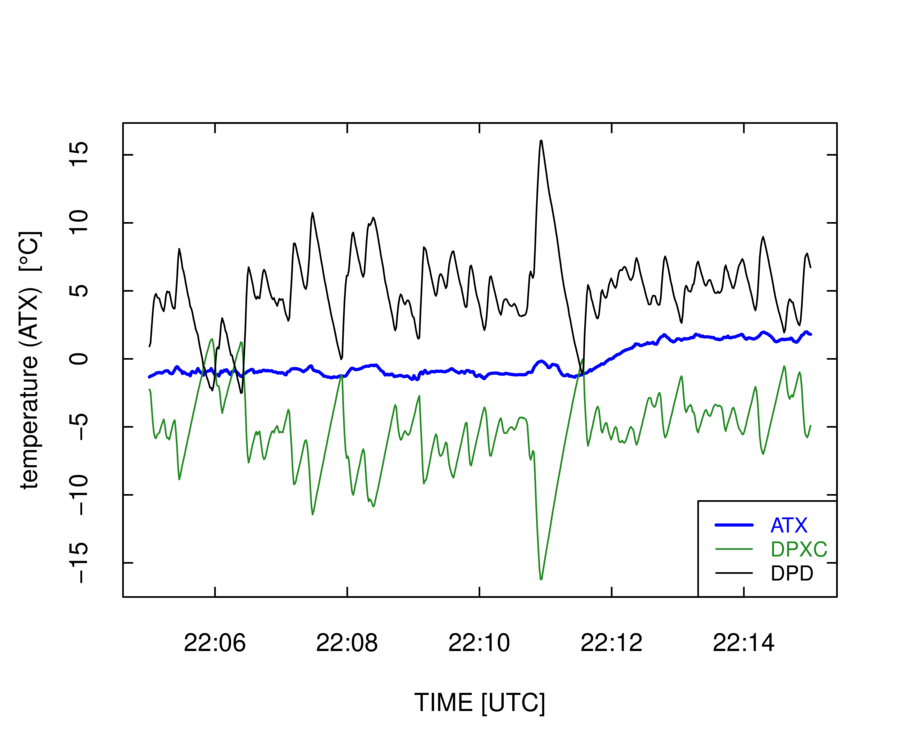
\includegraphics[width=\maxwidth]{figure/pipe-example-1} 

}

\caption[Example of a figure generated using pipes]{Example of a figure generated using pipes. The variables are air temperature (ATX), dew point temperature (DPXC), and a new generated variable representing the dew point depression (DPD=ATX-DPXC). From WECAN research flight 6, 3 August 2018.}\label{fig:pipe-example}
\end{figure}


\end{knitrout}

More information on some of the utility functions used or available
when constructing plots is provided in the following list:
\begin{enumerate}
\item \texttt{dplyr::filter(): }This function is used to limit the range
of accepted values. The arguments are a data.frame (provided above
by the pipe) and a logical statement. Only rows for which the specified
test is true are included in the resulting data.frame. An example
where a statement like this might be useful is when fitting to determine
the sensitivity coefficients for angle of attack, because it is useful
to exclude slow flight when the gear and/or flaps might be deployed.
Be sure to use the version from dplyr; the filter functions from the
packages ``stats'' or ``signal'' have different behavior. An alternative
method of creating a subset is to use the notation ``Data{[}Data\$TASX
> 90, {]}''. The disadvantage of this method and of the ``select(Data,
Data\$TASX > 90)'' function provided by base-R is that variable attributes
are lost.\footnote{Preserving attributes is desirable because the attributes are often
used by Ranadu routines. The bin assignments for size distributions
are carried in an attribute, as is the data rate (used in spectral
analysis). Variables with the same ``short\_name'' attributes are
redundant measurements of the same quantity, so it is often useful
to plot all with matching short\_names together. RANADU plot routines
use a ``label'' attribute for default axes titles. Finally, the
function makeNetCDF( ) makes a new netCDF file with the variables
and attributes in the data.frame, and it requires some attributes
(like the ``Dimension'' attribute) or it will fail.}
\item \texttt{dplyr::select(): }This function creates a subset data.frame
with only the desired variables. The desired list of names can be
specified either as character names (with quotes) or variable names
(without quotes). This also has the advantage over the ``{[}{]}''
or ``{[}{[}{]}{]}'' methods of subsetting that attributes of the
data.frame and the variables are preserved.
\item \texttt{Ranadu::Rmutate( ):} This function adds new variables to the
data.frame according to formulas specified in the second argument.
In this processing chain, the first argument is the data.frame provided
by the pipe. This calls the routine \texttt{dplyr::mutate()} but then,
because that function does not preserve variable attributes, it transfers
attributes from the input to the output data.frame. New variables,
however, have no attributes (even the ``Dimension'' attribute) so
the resulting data.frame has some limitations, notably not being accepted
by ``makeNetCDF( )'' unless the required attributes are added.
\item \texttt{Ranadu::selectTime( ): }This function limits the time range
of the resulting data.frame to be between the times that are specified
in HHMMSS format (hours, minutes, seconds). This is equivalent to
using ``dplyr::filter( )'' with limits on the accepted times, but
it avoids the need to provide those times in the POSIXct format used
by Ranadu data.frames. It preserves attributes and is suitable for
use in pipes.
\item \texttt{Ranadu::Rsubset( ): }This is not used in the present example
but could be. It accepts start and end times like ``selectTime'',
selects variables like ``dplyr::select'', and imposes limitations
on the data like ``dplyr::filter( )'', so several functions could
be combined in one step: Ranadu::getNetCDF(fname, Variables) \%>\%
Ranadu::Rsubset(220500, 221500, c('ATX', 'DPXC')) \%>\% plotWAC( ).
This function also preserves attributes in the modified data.frame.
\end{enumerate}
``Ranadu::plotWAC( )'' is designed primarily for time-series plots,
but scatterplots can also be generated. In that case, the first two
variables in the data.frame should be the variables for the scatterplot,
not the Time variable, and an explicit label ``xlab=xxx'' must be
supplied to override the default ``Time'' abscissa. Here is an example:

\begin{knitrout}
\definecolor{shadecolor}{rgb}{0.969, 0.969, 0.969}\color{fgcolor}\begin{kframe}
\begin{alltt}
\hlstd{Data} \hlopt \hlkwd{selectTime}\hlstd{(}\hlnum{220000}\hlstd{,} \hlnum{221500}\hlstd{)} \hlopt
         \hlstd{dplyr}\hlopt{::}\hlkwd{select}\hlstd{(ATX, DPXC)} \hlopt
         \hlkwd{plotWAC}\hlstd{(}\hlkwc{xlab}\hlstd{=}\hlstr{'ATX'}\hlstd{,} \hlkwc{type}\hlstd{=}\hlstr{'p'}\hlstd{)}
\end{alltt}
\end{kframe}\begin{figure}

{\centering 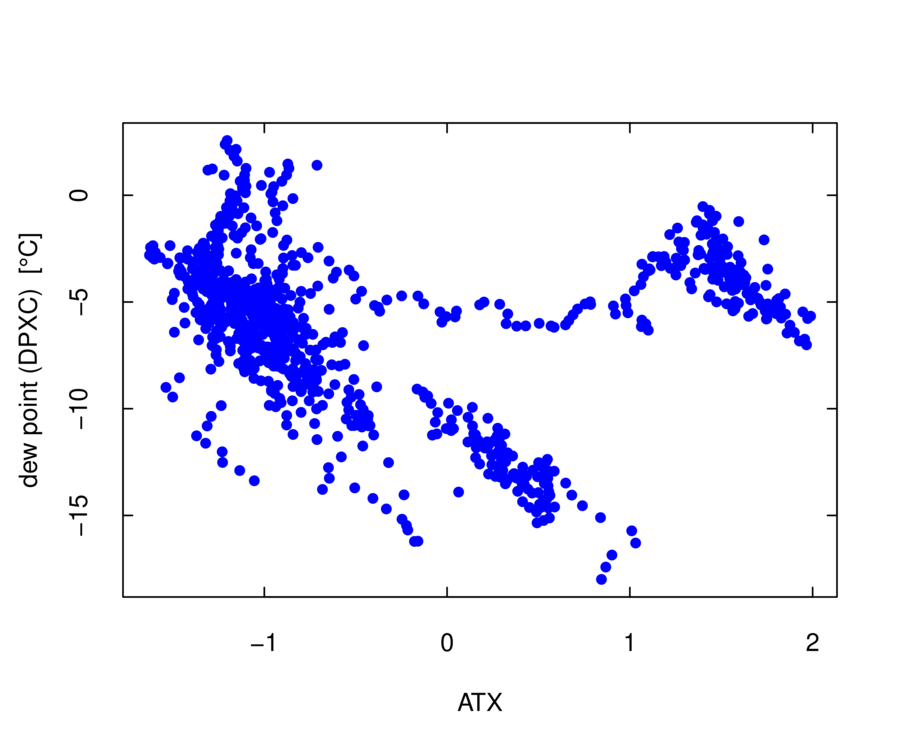
\includegraphics[width=\maxwidth]{figure/scat-ex-1} 

}

\caption[Example scatterplot]{Example scatterplot.}\label{fig:scat-ex}
\end{figure}


\end{knitrout}

\section{Multi-Frame Plots}

It is often desirable to combine several plots into a single plot.
There are several ways to do this with Ranadu routines:

\subsection{Multiple plotWAC( ) plots:}

The ``layout()'' function in base-R can be used. Here is an example.\footnote{The matrix layout can also be used to display plots in multiple columns
or in multiple rows and columns.}

\begin{knitrout}
\definecolor{shadecolor}{rgb}{0.969, 0.969, 0.969}\color{fgcolor}\begin{kframe}
\begin{alltt}
\hlkwd{layout}\hlstd{(}\hlkwd{matrix}\hlstd{(}\hlnum{1}\hlopt{:}\hlnum{2}\hlstd{,} \hlkwc{ncol}\hlstd{=}\hlnum{1}\hlstd{),} \hlkwc{widths}\hlstd{=}\hlkwd{c}\hlstd{(}\hlnum{8}\hlstd{,}\hlnum{8}\hlstd{),} \hlkwc{heights}\hlstd{=}\hlkwd{c}\hlstd{(}\hlnum{5.5}\hlstd{,}\hlnum{8}\hlstd{))}
\hlstd{op} \hlkwb{<-} \hlkwd{par} \hlstd{(}\hlkwc{mar}\hlstd{=}\hlkwd{c}\hlstd{(}\hlnum{2}\hlstd{,}\hlnum{4}\hlstd{,}\hlnum{1}\hlstd{,}\hlnum{1}\hlstd{)}\hlopt{+}\hlnum{0.1}\hlstd{,} \hlkwc{oma}\hlstd{=}\hlkwd{c}\hlstd{(}\hlnum{1.1}\hlstd{,}\hlnum{0}\hlstd{,}\hlnum{0}\hlstd{,}\hlnum{0}\hlstd{))}
\hlstd{Data} \hlopt \hlstd{dplyr}\hlopt{::}\hlkwd{select}\hlstd{(Time, ATX)} \hlopt
         \hlkwd{plotWAC}\hlstd{(}\hlkwc{ylab}\hlstd{=}\hlkwd{expression}\hlstd{(}\hlkwd{paste}\hlstd{(}\hlstr{"T ["}\hlstd{, degree,} \hlstr{"C]"}\hlstd{)))}
\hlstd{op} \hlkwb{<-} \hlkwd{par} \hlstd{(}\hlkwc{mar}\hlstd{=}\hlkwd{c}\hlstd{(}\hlnum{5}\hlstd{,}\hlnum{4}\hlstd{,}\hlnum{1}\hlstd{,}\hlnum{1}\hlstd{)}\hlopt{+}\hlnum{0.1}\hlstd{)}
\hlstd{Data} \hlopt \hlstd{dplyr}\hlopt{::}\hlkwd{select}\hlstd{(Time, WIC)} \hlopt
         \hlkwd{plotWAC}\hlstd{(}\hlkwc{ylab}\hlstd{=}\hlkwd{expression}\hlstd{(}\hlkwd{paste}\hlstd{(}\hlstr{'W [m/s]'}\hlstd{)))}
\end{alltt}
\end{kframe}\begin{figure}

{\centering 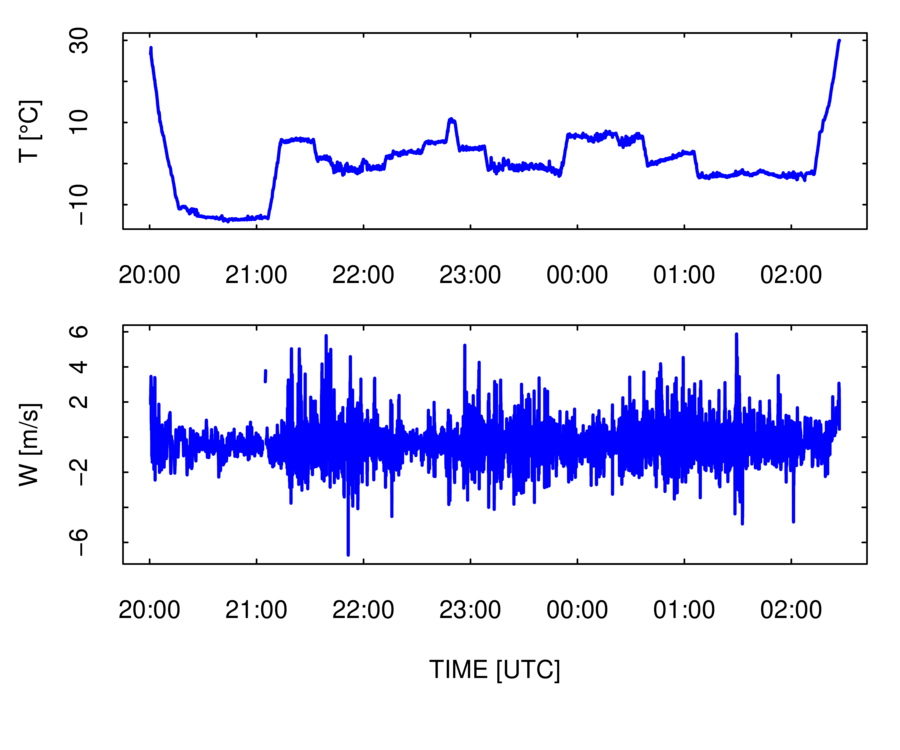
\includegraphics[width=\maxwidth]{figure/layout-example-1} 

}

\caption[Two-panel figure]{Two-panel figure.}\label{fig:layout-example}
\end{figure}


\end{knitrout}



\subsection{Panels and Facets in ggplotWAC( ):}

The function \texttt{Ranadu::ggplotWAC( )} is based on the ggplot2
package for R, which provides extensive plotting capabilities and
is highly recommended. What is provided via ggplotWAC( ) is a very
simplified and restricted approach, but it might be useful in preliminary
applications. See \href{http://had.co.nz/ggplot2/}{this URL} for
information on ggplot2. The Ranadu routine provides two approaches
to multiple plots:
\begin{itemize}
\item ``\uline{facets}'': If the argument ``panels'' is supplied
(e.g., panels=N), ggplotWAC( ) will construct N vertically aligned
panels. All will contain time-series plots. The first-argument to
ggplotWAC(), the data.frame, should contain the variable ``Time''
and N{*}M variables, where the first M variables will be plotted in
the first panel, the next M in the second panel, etc. A set of M character-mode
labels should be supplied via labelN.
\item ``\uline{viewports}'': An optional argument ``position=c(i,
j)'' can be used to place a plot in the ith of j vertically aligned
viewports.
\end{itemize}
Examples are shown in Figs.~\ref{fig:gg-facets} and \ref{fig:gg-viewports}.
An advantage of the faceted plot is that vertical alignment of the
plots is ensured; this can be a problem with other plots if the axis
labels are of different size in the different plots.\footnote{``suppressWarnings'' is used here because otherwise the routine
prints a warning message about mismatches among variable attributes.} In both cases, the viewports are positioned so that the abscissa
labels and title are obscured for the top plot. The intent is that
this should be used for identical time scales for each plot, so that
it is not necessary to duplicate the axis labels and title.

\begin{knitrout}
\definecolor{shadecolor}{rgb}{0.969, 0.969, 0.969}\color{fgcolor}\begin{kframe}
\begin{alltt}
\hlstd{Project} \hlkwb{<-} \hlstr{'WECAN'}    \hlcom{## faceted plot with ggplotWAC()}
\hlstd{Flight} \hlkwb{<-} \hlnum{5}
\hlstd{V} \hlkwb{<-} \hlkwd{c}\hlstd{(}\hlstr{'ATH1'}\hlstd{,} \hlstr{'ATH2'}\hlstd{,} \hlstr{'ATF1'}\hlstd{,} \hlstr{'RTH1'}\hlstd{,} \hlstr{'RTH2'}\hlstd{,} \hlstr{'RTF1'}\hlstd{)}
\hlstd{fname} \hlkwb{<-} \hlkwd{sprintf}\hlstd{(}\hlstr{'%s%s/%srf%02d.nc'}\hlstd{,} \hlkwd{DataDirectory}\hlstd{(), Project, Project,}
                 \hlstd{Flight)}
\hlkwd{suppressWarnings} \hlstd{(}
    \hlkwd{getNetCDF}\hlstd{(fname, V,} \hlnum{200000}\hlstd{,} \hlnum{201500}\hlstd{)} \hlopt
    \hlkwd{ggplotWAC}\hlstd{(}\hlkwc{panels}\hlstd{=}\hlnum{2}\hlstd{,}
              \hlkwc{col}\hlstd{=}\hlkwd{c}\hlstd{(}\hlstr{'blue'}\hlstd{,} \hlstr{'darkorange'}\hlstd{,} \hlstr{'forestgreen'}\hlstd{),}
              \hlkwc{ylab}\hlstd{=}\hlkwd{expression}\hlstd{(}\hlkwd{paste}\hlstd{(}\hlstr{'temperature ['}\hlstd{, degree,}\hlstr{'C]'}\hlstd{)),}
              \hlkwc{lwd}\hlstd{=}\hlkwd{c}\hlstd{(}\hlnum{1.5}\hlstd{,} \hlnum{0.8}\hlstd{,} \hlnum{1}\hlstd{),} \hlkwc{lty}\hlstd{=}\hlkwd{c}\hlstd{(}\hlnum{1}\hlstd{,}\hlnum{2}\hlstd{,}\hlnum{1}\hlstd{),}
              \hlkwc{labelP}\hlstd{=}\hlkwd{c}\hlstd{(}\hlstr{'   air temperature'}\hlstd{,} \hlstr{' recovery temperature'}\hlstd{),}
              \hlkwc{labelL}\hlstd{=}\hlkwd{c}\hlstd{(}\hlstr{'H1'}\hlstd{,} \hlstr{'H2'}\hlstd{,} \hlstr{'F1'}\hlstd{),}
              \hlkwc{legend.position}\hlstd{=}\hlkwd{c}\hlstd{(}\hlnum{0.5}\hlstd{,}\hlnum{0.95}\hlstd{)}
    \hlstd{)}
\hlstd{)}
\end{alltt}
\end{kframe}\begin{figure}

{\centering 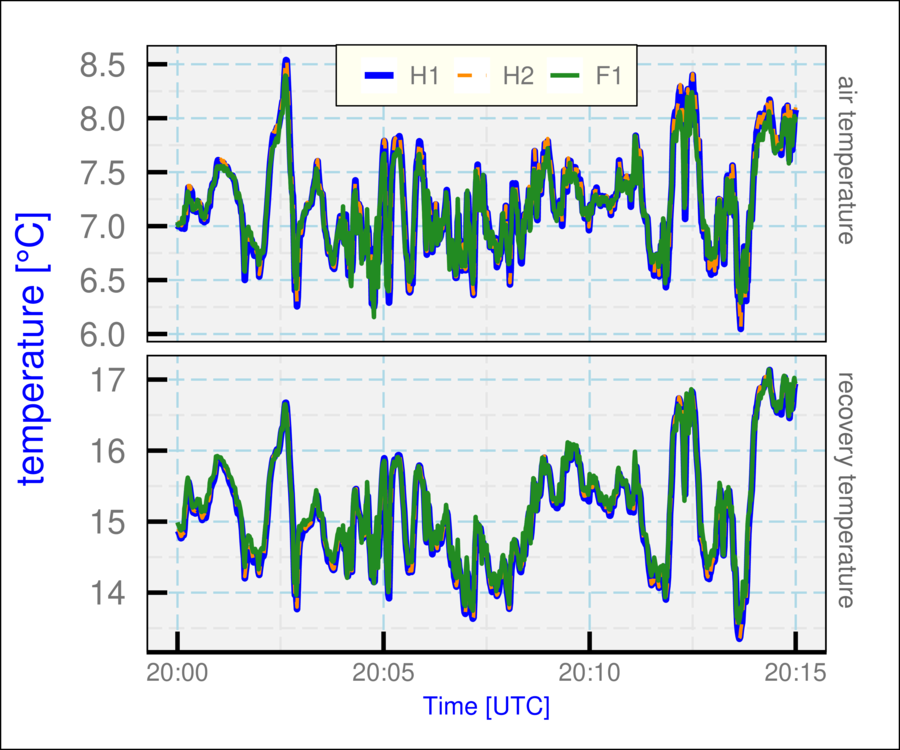
\includegraphics[width=\maxwidth]{figure/gg-facets-1} 

}

\caption[Example of a faceted ggplotWAC plot]{Example of a faceted ggplotWAC plot. Three temperature measurements are shown from probes identified as H1, H2, and F2. The top panel shows the air temperature, and the bottom panel the directly measured recovery temperature before correction for dynamic heating.}\label{fig:gg-facets}
\end{figure}


\end{knitrout}

\pagebreak{}

\begin{knitrout}
\definecolor{shadecolor}{rgb}{0.969, 0.969, 0.969}\color{fgcolor}\begin{kframe}
\begin{alltt}
\hlcom{## viewport-plot with ggplotWAC()}
\hlstd{DG} \hlkwb{<-} \hlkwd{getNetCDF}\hlstd{(fname, V,} \hlnum{200000}\hlstd{,} \hlnum{201500}\hlstd{)}
\hlkwd{with}\hlstd{(DG,} \hlkwd{ggplotWAC}\hlstd{(}\hlkwd{data.frame}\hlstd{(Time, ATH1),} \hlkwc{position}\hlstd{=}\hlkwd{c}\hlstd{(}\hlnum{1}\hlstd{,}\hlnum{2}\hlstd{)))}
\hlkwd{with}\hlstd{(DG,} \hlkwd{ggplotWAC}\hlstd{(}\hlkwd{data.frame}\hlstd{(Time, ATF1),} \hlkwc{position}\hlstd{=}\hlkwd{c}\hlstd{(}\hlnum{2}\hlstd{,}\hlnum{2}\hlstd{)))}
\end{alltt}
\end{kframe}\begin{figure}

{\centering 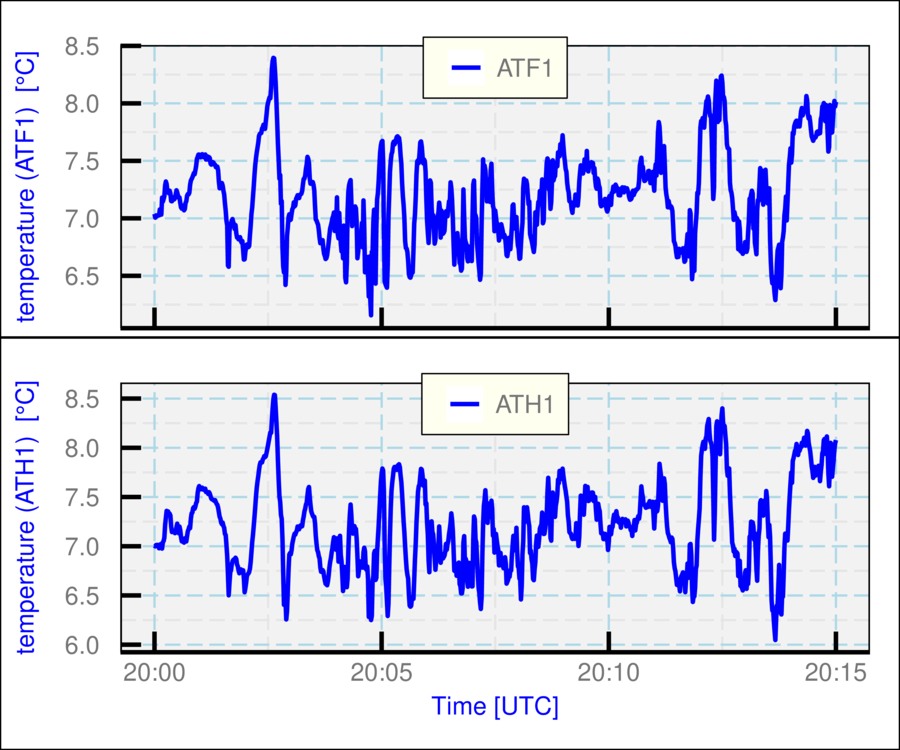
\includegraphics[width=\maxwidth]{figure/gg-viewports-1} 

}

\caption[An example of selecting the figure position using viewports and the "position" argument to ggplotWAC()]{An example of selecting the figure position using viewports and the "position" argument to ggplotWAC().}\label{fig:gg-viewports}
\end{figure}


\end{knitrout}

\pagebreak{}

\section{Plotting the density of events}

A scatterplot like that in Fig.~\ref{fig:scat-ex} often is used
to show a two-dimensional display of where events occur. Such plots
are useful when the number of events is small, but for large numbers
of events the overlap of points can obscure relationships. The base-R
function ``smoothScatter()'' is one option for plotting the density
of points in such cases. Another is the ``filled.contour()'' function.
Ranadu provides a third option in the function Ranadu::contourPlot().
The number of bins, colors, and linear vs.~logarithmic density intervals
can be provided as arguments to this function, although the defaults
often work acceptably. The following figure and code illustrates the
use of this plot. Additional more elegant solutions are provided by
the ggplot2 package.

\begin{knitrout}
\definecolor{shadecolor}{rgb}{0.969, 0.969, 0.969}\color{fgcolor}\begin{kframe}
\begin{alltt}
\hlkwd{getNetCDF}\hlstd{(fname)} \hlopt \hlstd{dplyr}\hlopt{::}\hlkwd{select}\hlstd{(ATX, DPXC)} \hlopt
    \hlkwd{contourPlot}\hlstd{(}\hlkwc{title}\hlstd{=}\hlstr{'WECAN flight #5'}\hlstd{)}
\end{alltt}
\end{kframe}\begin{figure}

{\centering 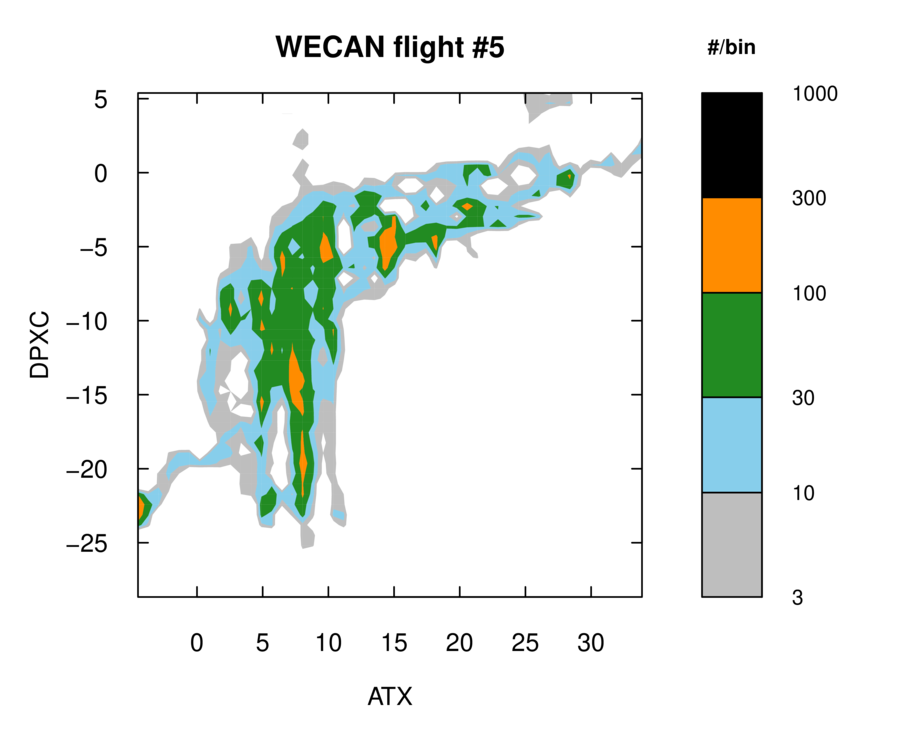
\includegraphics[width=\maxwidth]{figure/contourPlot-1} 

}

\caption[Example of a density plot generated using Ranadu::contourPlot()]{Example of a density plot generated using Ranadu::contourPlot().}\label{fig:contourPlot}
\end{figure}


\end{knitrout}

\pagebreak{}

\section{Error bars and box-and-whisker plots}

Ranadu provides the ``binStats()'' function to compile variable
characteristics needed to generate plots like error-bar plots and
box-and-whisker plots. The input should be a data.frame whose first
two columns specify the expected respective ordinate and abscissa
variables. Each row in the data.frame is assigned to a bin on the
basis of the value of the second variable, and for each bin the mean,
standard deviation, and number of events are accumulated for values
of the first variable in the data.frame. The output from binStats()
is a new four-column data.frame where the respective columns are the
mean value of the abscissa for each bin, the mean value of the ordinate
for all events in the bin, and corresponding standard deviation, and
the number of events in the bin.

\begin{knitrout}
\definecolor{shadecolor}{rgb}{0.969, 0.969, 0.969}\color{fgcolor}\begin{kframe}
\begin{alltt}
\hlkwd{getNetCDF}\hlstd{(fname)} \hlopt
  \hlkwd{Rmutate}\hlstd{(}\hlkwc{DPD}\hlstd{=ATX}\hlopt{-}\hlstd{DPXC)} \hlopt      \hlcom{## define dew-point-depression variable}
  \hlstd{dplyr}\hlopt{::}\hlkwd{select}\hlstd{(DPD, GGALT)} \hlopt
  \hlkwd{binStats}\hlstd{()} \hlopt
  \hlkwd{ggplot}\hlstd{(}\hlkwd{aes}\hlstd{(}\hlkwc{x}\hlstd{=xc))} \hlopt{+} \hlkwd{geom_point}\hlstd{(}\hlkwd{aes}\hlstd{(}\hlkwc{y}\hlstd{=ybar),} \hlkwc{color}\hlstd{=}\hlstr{'blue'}\hlstd{)} \hlopt{+}
  \hlkwd{geom_errorbar}\hlstd{(}\hlkwd{aes}\hlstd{(}\hlkwc{ymin}\hlstd{=ybar}\hlopt{-}\hlstd{sigma,} \hlkwc{ymax}\hlstd{=ybar}\hlopt{+}\hlstd{sigma))} \hlopt{+}
  \hlkwd{xlab}\hlstd{(}\hlstr{'geometric altitude [m]'}\hlstd{)} \hlopt{+}
  \hlkwd{ylab}\hlstd{(}\hlkwd{expression}\hlstd{(}\hlkwd{paste}\hlstd{(}\hlstr{'dew point depression ['}\hlstd{, degree,} \hlstr{'C]'}\hlstd{)))} \hlopt{+}
  \hlkwd{theme_WAC}\hlstd{()}
\end{alltt}
\end{kframe}\begin{figure}

{\centering 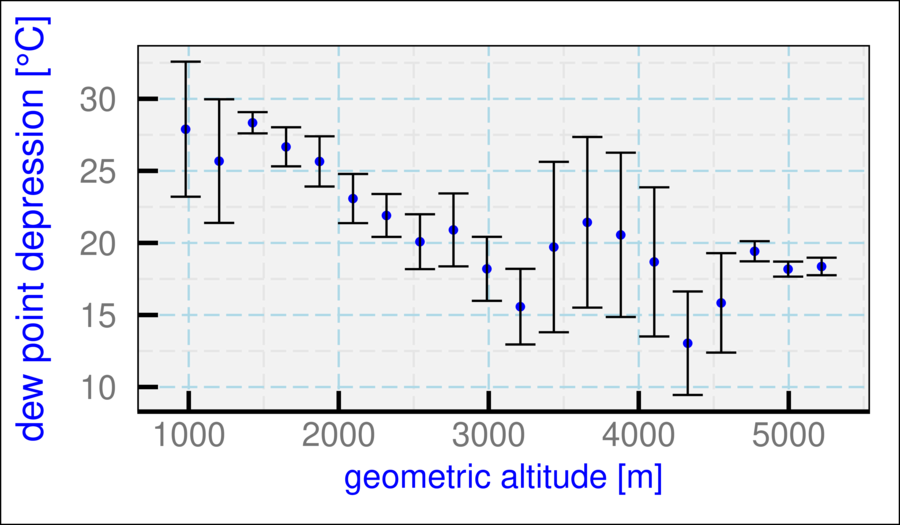
\includegraphics[width=\maxwidth]{figure/errorbar-plot-1} 

}

\caption[Example of an error-bar plot generated using binStats()]{Example of an error-bar plot generated using binStats().}\label{fig:errorbar-plot}
\end{figure}


\end{knitrout}

\pagebreak The following code creates Fig.~\ref{fig:bwplot}, an
example of creating a box-and-whisker plot. When used with the argument
``addBin = TRUE'', binStats instead returns a modified data.frame
with a variable ``BIN'' added that is suitable to use when grouping
in ggplot aesthetics.

\begin{knitrout}
\definecolor{shadecolor}{rgb}{0.969, 0.969, 0.969}\color{fgcolor}\begin{kframe}
\begin{alltt}
\hlkwd{getNetCDF}\hlstd{(fname)} \hlopt
  \hlstd{dplyr}\hlopt{::}\hlkwd{select}\hlstd{(DPXC, GGALT)} \hlopt
  \hlkwd{binStats}\hlstd{(}\hlkwc{addBin} \hlstd{=} \hlnum{TRUE}\hlstd{)} \hlopt
  \hlkwd{ggplot}\hlstd{()} \hlopt{+} \hlkwd{geom_boxplot}\hlstd{(}\hlkwd{aes}\hlstd{(GGALT, DPXC,} \hlkwc{group}\hlstd{=BIN),}
                          \hlkwc{color}\hlstd{=}\hlstr{'blue'}\hlstd{,} \hlkwc{na.rm}\hlstd{=}\hlnum{TRUE}\hlstd{)} \hlopt{+}
  \hlkwd{theme_WAC}\hlstd{()}
\end{alltt}
\end{kframe}\begin{figure}

{\centering 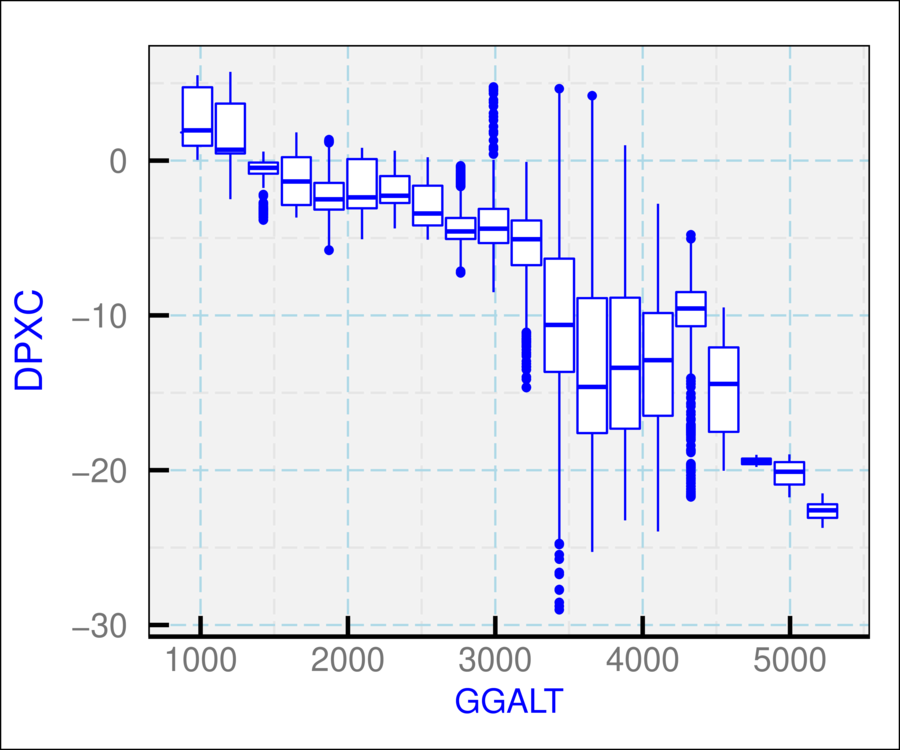
\includegraphics[width=\maxwidth]{figure/bwplot-1} 

}

\caption[An example of a box-and-whisker plot]{An example of a box-and-whisker plot.}\label{fig:bwplot}
\end{figure}


\end{knitrout}

\pagebreak{}

\section{The skew-T thermodynamic diagram}

Ranadu incorporates the ability to plot a set of measurements on the
background of a skew-T diagram. The background is non-standard and
is described in detail in \href{https://drive.google.com/file/d/0B1kIUH45ca5ANVNoMnowUlhpYk0/view?usp=sharing}{this document}.
The ``Ranadu::SkewTSounding()'' function should be called with a
data.frame containing measurements of pressure, temperature and dewpoint,
which may be named either (``PSXC'', ``ATX'', ``DPXC'') or (``Pressure'',
``Temperature'', ``DewPoint''). A skew-T background is generated
using the Ranadu data file ``skewTDiagram.Rdata'' and the values
from the input data.frame are optionally averaged in pressure intervals
and then plotted on this background.

\begin{knitrout}
\definecolor{shadecolor}{rgb}{0.969, 0.969, 0.969}\color{fgcolor}\begin{kframe}
\begin{alltt}
\hlstd{Project} \hlkwb{<-} \hlstr{'PREDICT'}
\hlstd{Flight} \hlkwb{<-} \hlnum{11}
\hlstd{fname} \hlkwb{<-} \hlkwd{sprintf} \hlstd{(}\hlstr{'%s%s/%srf%02d.nc'}\hlstd{,} \hlkwd{DataDirectory}\hlstd{(), Project,}
                  \hlstd{Project, Flight)}
\hlkwd{getNetCDF}\hlstd{(fname)} \hlopt
    \hlkwd{selectTime}\hlstd{(}\hlnum{0}\hlstd{,} \hlnum{150000}\hlstd{)} \hlopt
    \hlkwd{SkewTSounding}\hlstd{(}\hlkwc{AverageInterval}\hlstd{=}\hlnum{10}\hlstd{)}
\end{alltt}
\end{kframe}\begin{figure}

{\centering 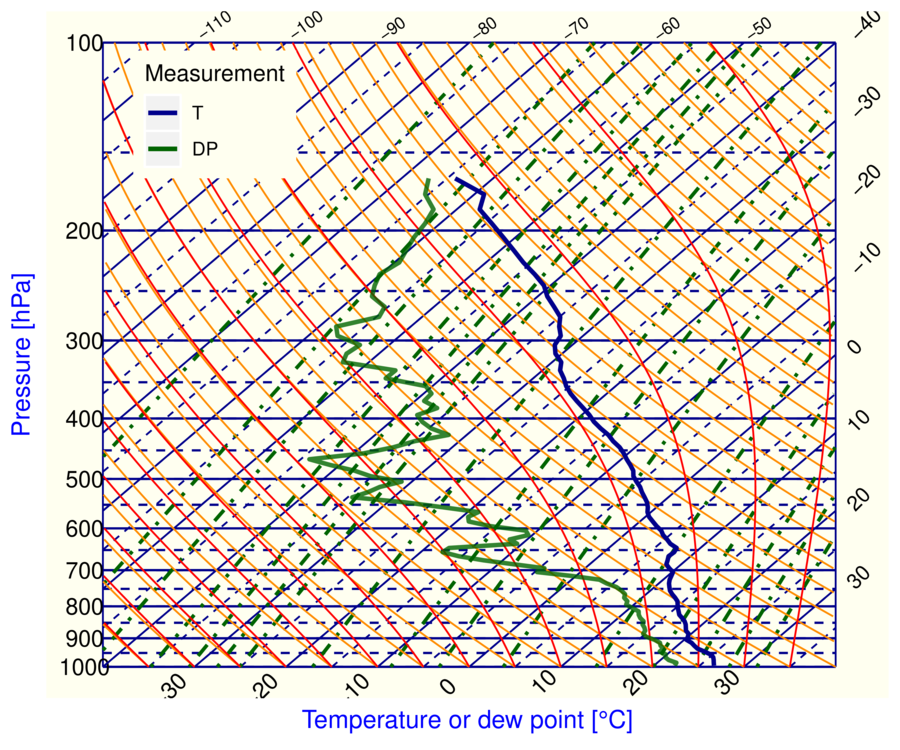
\includegraphics[width=\maxwidth]{figure/skewT-1} 

}

\caption[Sounding from PREDICT flight 11]{Sounding from PREDICT flight 11.}\label{fig:skewT}
\end{figure}


\end{knitrout}

\section{Aerosol- and hydrometeor-size distributions}

The Ranadu function ``plotSD()'' displays the size distribution
measured by various probes that produce arrays of measurements. The
data.frame containing these measurements is special in that the column
corresponding to a variable name like ``CCDP\_RPC'' is a two-dimensional
vector. This makes the data.frame inconsistent with the ``tidy''
structure and with the structure required for a ``tibble'', so some
special considerations are required if an analyst wants to use only
tidy data. In this section, those considerations are not discussed
further because the ``plotSD()'' function assumes Ranadu-style data.frame
conventions.

``Ranadu::getNetCDF()'' accepts variable names like ``CCDP\_'',
in which case it searches for the first variable starting with that
name. This avoids the need to know the location of the CDP probe in
various projects. However, if there are multiple probes with the same
prefix name, they need to be specified in the variable list used to
construct the data.frame.

An example, Fig.~\ref{fig:SD1}, shows code that will construct a
plot of the size distribution from several probes. The ``exceedance''
is added when the argument ``CDF=TRUE'' is used; it is the complement
to a cumulative distribution and shows the fraction of particles that
exceed the plotted size. The four numbers returned from the function
are the mean concentration, mean diameter, standard deviation in the
diameter, and liquid water content under the assumption that all particles
are liquid. It is also possible to construct a plot of the distribution
in liquid water content, as shown in Fig.~\ref{fig:SD2}. See ``?Ranadu::plotSD''
for more options including alternate specification of the size limits,
bins to include, and log vs linear axes.

\begin{knitrout}
\definecolor{shadecolor}{rgb}{0.969, 0.969, 0.969}\color{fgcolor}\begin{kframe}
\begin{alltt}
\hlkwd{getNetCDF}\hlstd{(}\hlstr{'/Data/CSET/CSETrf06.nc'}\hlstd{,} \hlkwd{c}\hlstd{(}\hlstr{'CCDP_'}\hlstd{,} \hlstr{'C1DC_'}\hlstd{,} \hlstr{'CUHSAS_'}\hlstd{))} \hlopt
  \hlkwd{selectTime}\hlstd{(}\hlnum{173000}\hlstd{,} \hlnum{173500}\hlstd{)} \hlopt
  \hlkwd{plotSD}\hlstd{(}\hlkwc{CellLimits}\hlstd{=}\hlnum{NA}\hlstd{,} \hlkwc{logAxis}\hlstd{=}\hlstr{'xy'}\hlstd{,} \hlkwc{CDF}\hlstd{=}\hlnum{TRUE}\hlstd{)}
\end{alltt}
\end{kframe}\begin{figure}

{\centering 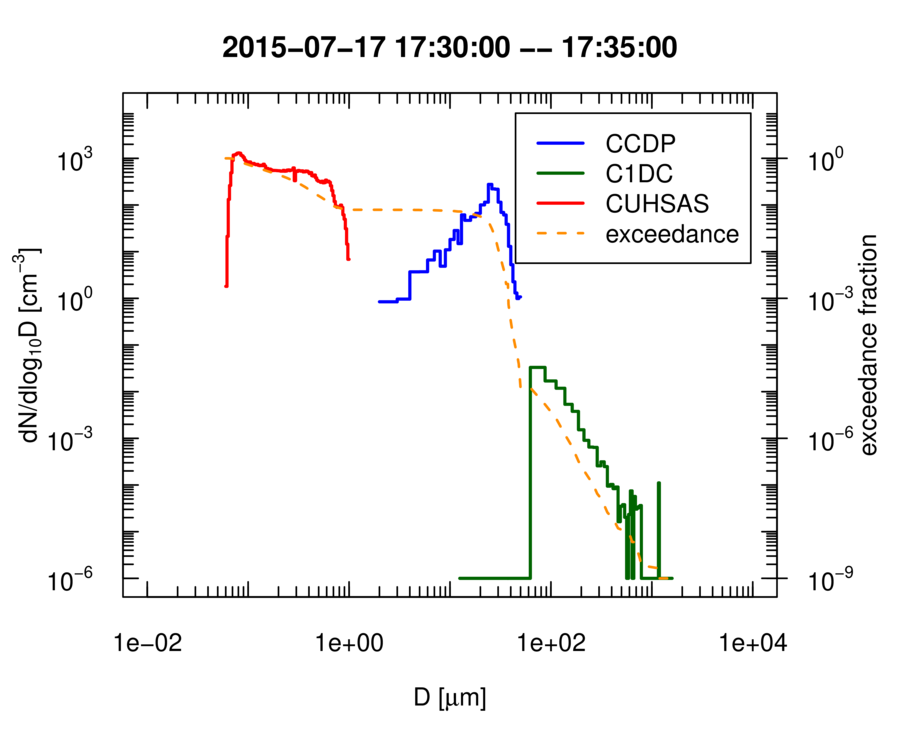
\includegraphics[width=\maxwidth]{figure/SD1-1} 

}

\caption[Example of a size distribution]{Example of a size distribution.}\label{fig:SD1}
\end{figure}

\begin{kframe}\begin{verbatim}
## [1] 700.6157510   2.0525220   7.2263178   0.4802542
\end{verbatim}
\end{kframe}
\end{knitrout}

\pagebreak{}

\begin{knitrout}
\definecolor{shadecolor}{rgb}{0.969, 0.969, 0.969}\color{fgcolor}\begin{kframe}
\begin{alltt}
\hlkwd{getNetCDF}\hlstd{(}\hlstr{'/Data/CSET/CSETrf06.nc'}\hlstd{,} \hlkwd{c}\hlstd{(}\hlstr{'CCDP_'}\hlstd{,} \hlstr{'C1DC_'}\hlstd{,} \hlstr{'CUHSAS_'}\hlstd{))} \hlopt
  \hlkwd{selectTime}\hlstd{(}\hlnum{173000}\hlstd{,} \hlnum{173500}\hlstd{)} \hlopt
  \hlkwd{plotSD}\hlstd{(}\hlkwc{CellLimits}\hlstd{=}\hlnum{NA}\hlstd{,} \hlkwc{logAxis}\hlstd{=}\hlstr{'xy'}\hlstd{,} \hlkwc{LWC}\hlstd{=}\hlnum{TRUE}\hlstd{,} \hlkwc{CDF}\hlstd{=}\hlnum{TRUE}\hlstd{)}
\end{alltt}
\end{kframe}\begin{figure}

{\centering 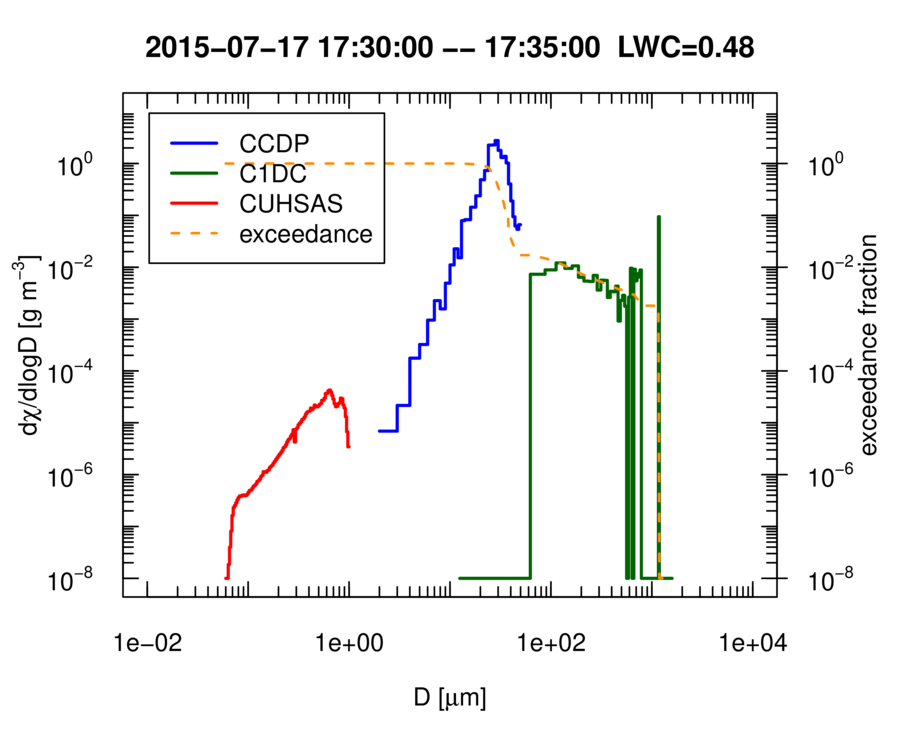
\includegraphics[width=\maxwidth]{figure/SD2-1} 

}

\caption[Example of a distribution in liquid water content]{Example of a distribution in liquid water content.}\label{fig:SD2}
\end{figure}

\begin{kframe}\begin{verbatim}
## [1] 700.6157510   2.0525220   7.2263178   0.4802542
\end{verbatim}
\end{kframe}
\end{knitrout}

\chapter{Variance Spectra}

Variance spectra are also plots and perhaps belong in the preceding
chapter, but they are discussed here in greater detail than the preceding
plots and so seemed to fit better in a separate chapter.

\section{Background regarding spectral variance}

\subsection{Terminology}

The plots discussed here as ``variance spectra'' are often referred
to as ``power spectra.'' That term is not used here because the
spectra representing variance in the data.frame measurements from
NCAR/EOL/RAF netCDF files are not power. Even in the case of wind
(with variance dimensions $\mathrm{m}^{2}\mathrm{s}^{-1}/Hz$), the
variance spectrum is better described as a kinetic-energy spectrum.
For this reason, the plots discussed in this chapter will be called
``variance spectra'' and the plotted quantity will be called the
spectral variance.

\subsection{Transformations among spectra; ``proper'' spectra}

Consider the cumulative distribution function for variance $C(\nu)$,
the fraction of the variance that is contributed by frequencies smaller
than $\nu$. The differential distribution function with respect to
frequency is then
\[
P(\nu)=\frac{dC(\nu)}{d\nu}\,\,\,\,.
\]
Consider how this distribution function would change if defined in
terms of a new variable $x(v)$ starting with the specific variable
$x=\ln\nu$. The differential distribution function would then be
$T(x)$ specified by\\
\[
T(x)=\frac{dC(x)}{dx}=\frac{dC(\nu)}{d\nu}\frac{d\nu}{dx}=\nu P(\nu)
\]
$\nu P(\nu)$ thus gives the spectral density in terms of $\ln\nu$
and so in terms of $\ln(10)\log_{10}\nu\approx2.30\log_{10}\nu$.
In the following, two options for variance spectra are emphasized:
$P(\nu)$ vs $\nu$ on a linear plot and $\nu P(\nu)$ vs $\log_{10}\nu$
with a logarithmic abscissa and either a linear or logarithmic ordinate
scale. These are regarded here as ``proper'' displays because the
area under segments of the plotted curves represent contributions
to the variance so it is possible to estimate the contributions to
variance from various intervals in frequency by using the areas on
the plot. This direct representation is compromised in the case where
the variable $\nu P(\nu)$ is plotted on a logarithmic scale because
then it is necessary to consider the logarithmic ordinate when evaluating
areas. This minor inconvenience nevertheless is less significant than
the problems that arise from using a linear ordinate scale, in which
case the ordinate range obscures relationships and the common ``$-5/3$''
slope seen in logarithmic plots becomes a parabolic line that is difficult
to interpret. For that reason, plots of spectral variance here will
emphasis plots of $\nu P(\nu)$ vs $\log_{10}(\nu)$ on log-log scales.
It is suggested that plots of $P(\nu)$ vs $\nu$ on log-log scales
should be avoided because the connection between area on the plot
and variance is lost, making the plot harder to interpret. In addition,
``$-5/3$'' spectra are steep, the range of ordinate values is higher,
and the plots are therefore more difficult to interpret than those
plotting $\nu P(\nu)$ vs $\nu$ on a log-log scale.

\subsection{Methods used to estimate spectral variance}

The function ``Ranadu::VSpec()'' includes three methods that can
be selected to estimate the spectral variance:
\begin{enumerate}
\item The function ``spectrum()'' from the ``stats'' R package, which
estimates a periodogram using Fourier-series estimation and then optionally
smooths the spectrum using modified Daniell smoothers. The amount
of smoothing can be controlled with the ``spans'' parameter in the
function call.
\item The ``Welch'' method as implemented by the R package ``bspec''.
In this method, the time series is divided into subsets and the spectra
resulting from the subsets are averaged to reduce the variance in
the result. The degree of smoothing is controlled by the ``segLength''
parameter that specifies the length of the segments to use.
\item The ``maximum entropy'' method in which the spectrum is represented
by ``poles'' and evaluated from the contributions of those poles
across the frequency spectrum. A higher number of poles and a smaller
value of the ``resolution'' will lead to more structure in the result.
\end{enumerate}
In addition, it is possible to smooth the resulting spectrum further
by specifying a value for the parameter ``smoothBins'', in which
case the frequency range will be partitioned into the specified number
of logarithmically spaced bins and the values of the spectral density
will be averaged in each bin.

\pagebreak{}

\section{Generating plots of variance spectra}

See ``?Ranadu::VSpec'' for details regarding using this function.
The essential inputs are a data.frame that includes at least the variables
``Time'', ``TASX'', and the variable for which the variance spectrum
is desired. TASX is needed to interpret the scale both in terms of
frequency and wavelength. An example is shown in Fig.~\ref{fig:VS1},
using the default specifications.

\begin{knitrout}
\definecolor{shadecolor}{rgb}{0.969, 0.969, 0.969}\color{fgcolor}\begin{kframe}
\begin{alltt}
\hlkwd{getNetCDF}\hlstd{(}\hlstr{'/Data/SOCRATES/SOCRATESrf08h.nc'}\hlstd{,} \hlkwc{Start}\hlstd{=}\hlnum{45600}\hlstd{,} \hlkwc{End}\hlstd{=}\hlnum{50100}\hlstd{)} \hlopt
  \hlkwd{VSpec}\hlstd{(}\hlstr{'WIC'}\hlstd{)} \hlopt{+} \hlkwd{theme_WAC}\hlstd{()}
\end{alltt}
\end{kframe}\begin{figure}

{\centering 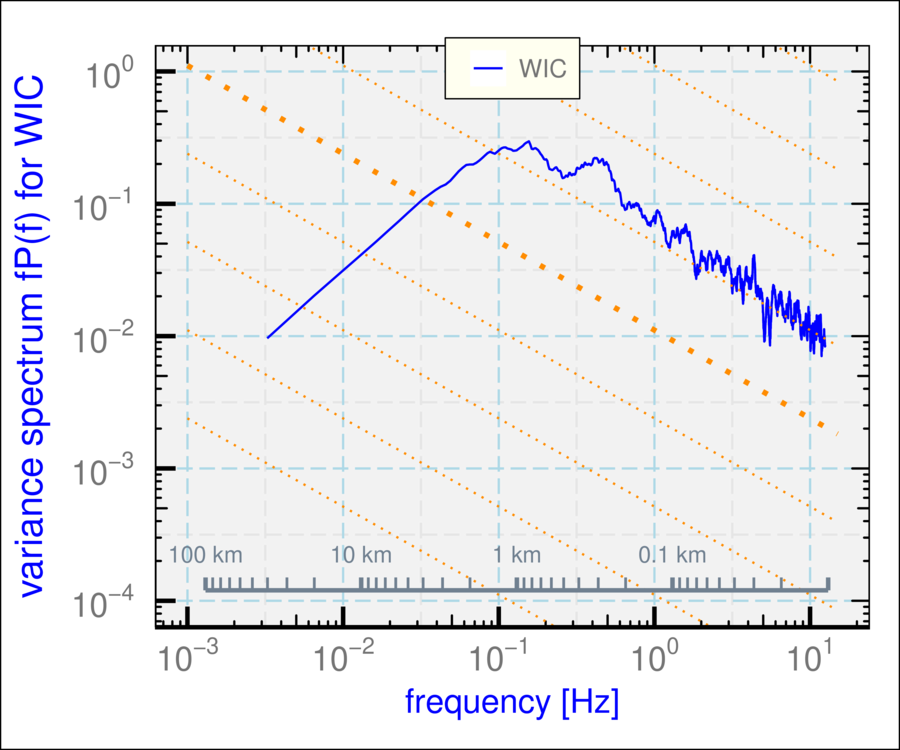
\includegraphics[width=\maxwidth]{figure/VS1-1} 

}

\caption[Variance spectrum for measurements of vertical wind during SOCRATES flight 8, 4:56:00 -- 5:01:00]{Variance spectrum for measurements of vertical wind during SOCRATES flight 8, 4:56:00 -- 5:01:00.}\label{fig:VS1}
\end{figure}


\end{knitrout}

The following demonstrates how to combine plotted spectra. The three
lines on this plot were generated using the three methods of spectral
estimation available in VSpec(), all for the WIC variable:

\begin{knitrout}
\definecolor{shadecolor}{rgb}{0.969, 0.969, 0.969}\color{fgcolor}\begin{kframe}
\begin{alltt}
\hlstd{D} \hlkwb{<-} \hlkwd{getNetCDF}\hlstd{(}\hlstr{'/Data/SOCRATES/SOCRATESrf08h.nc'}\hlstd{,} \hlkwc{Start}\hlstd{=}\hlnum{45600}\hlstd{,} \hlkwc{End}\hlstd{=}\hlnum{50100}\hlstd{)} \hlopt
     \hlkwd{Rmutate}\hlstd{(}\hlkwc{WIC2}\hlstd{=WIC,} \hlkwc{WIC3}\hlstd{=WIC)} \hlcom{## duplicate the variable}
\hlstd{g} \hlkwb{<-} \hlkwd{VSpec}\hlstd{(D,} \hlstr{'WIC'}\hlstd{,} \hlkwc{VLabel}\hlstd{=}\hlstr{'spectrum'}\hlstd{)}
\hlstd{g} \hlkwb{<-} \hlkwd{VSpec}\hlstd{(D,} \hlstr{'WIC2'}\hlstd{,} \hlkwc{method}\hlstd{=}\hlstr{'Welch'}\hlstd{,} \hlkwc{VLabel}\hlstd{=}\hlstr{'Welch'}\hlstd{,}
           \hlkwc{segLength}\hlstd{=}\hlnum{128}\hlstd{,} \hlkwc{smoothBins}\hlstd{=}\hlnum{50}\hlstd{,} \hlkwc{add}\hlstd{=g)}
\hlkwd{VSpec}\hlstd{(D,} \hlstr{'WIC3'}\hlstd{,} \hlkwc{method}\hlstd{=}\hlstr{'MEM'}\hlstd{,} \hlkwc{VLabel}\hlstd{=}\hlstr{'MEM'}\hlstd{,} \hlkwc{add}\hlstd{=g)} \hlopt{+}
  \hlkwd{theme_WAC}\hlstd{()}
\end{alltt}
\end{kframe}\begin{figure}

{\centering 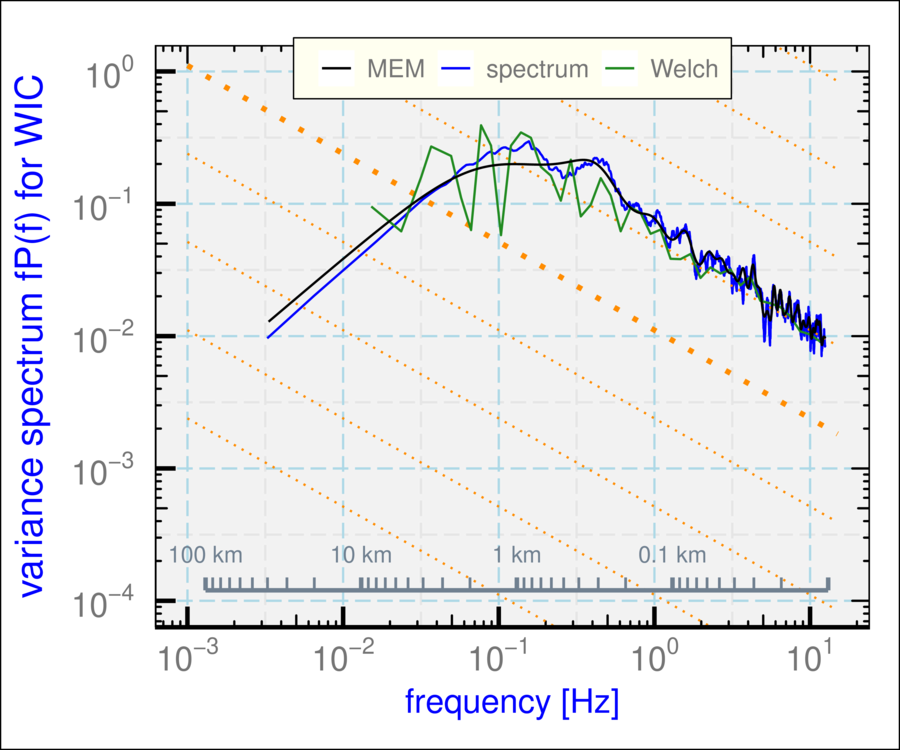
\includegraphics[width=\maxwidth]{figure/VS2-1} 

}

\caption[Variance spectra for the same data shown in the preceding plot but generated by the three methods indicated in the legend]{Variance spectra for the same data shown in the preceding plot but generated by the three methods indicated in the legend.}\label{fig:VS2}
\end{figure}


\end{knitrout}

\pagebreak{}

Another option that may be of use, although the result is not a ``proper''
spectrum in the sense used above, is to plot with weighting by $\nu^{5/3}$
and additional change of variables so that the resulting ordinate
matches the eddy dissipation rate in a case where the measurements
are indeed from an inertial subrange. Figure~\ref{fig:VS3} illustrates
this plot. The variable plotted is $(2\pi/V)(CP(\nu)\nu^{5/3})^{3/2}$,
with $V$ the airspeed and $C=1.5$ for lateral spectra; this quantity
should equal the eddy dissipation rate in an inertial subrange.

\begin{knitrout}
\definecolor{shadecolor}{rgb}{0.969, 0.969, 0.969}\color{fgcolor}\begin{kframe}
\begin{alltt}
\hlkwd{VSpec}\hlstd{(D,} \hlstr{'WIC'}\hlstd{,} \hlkwc{EDR}\hlstd{=}\hlnum{TRUE}\hlstd{)} \hlopt{+} \hlkwd{theme_WAC}\hlstd{(}\hlnum{1}\hlstd{)}  \hlcom{## theme_WAC(1) => smaller title}
\end{alltt}
\end{kframe}\begin{figure}

{\centering 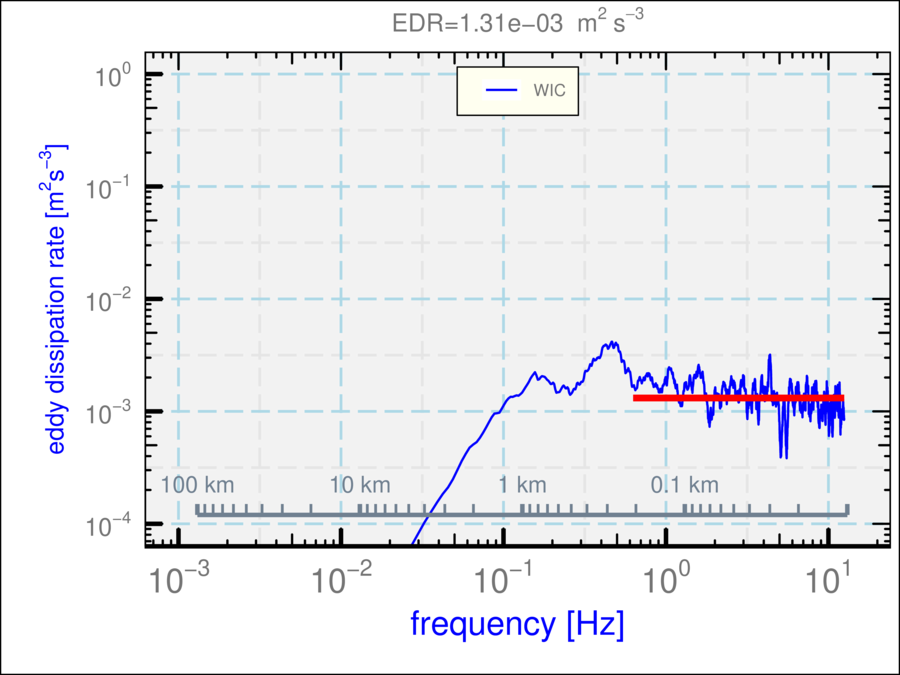
\includegraphics[width=\maxwidth]{figure/VS3-1} 

}

\caption[An eddy-dissipation-rate plot for the same data shown in the preceding plot]{An eddy-dissipation-rate plot for the same data shown in the preceding plot. but generated by the three methods indicated in the legend.}\label{fig:VS3}
\end{figure}

\begin{kframe}\begin{alltt}
\hlcom{## to suppress the title, add "+ ggtitle('')}
\end{alltt}
\end{kframe}
\end{knitrout}

\chapter{Miscellaneous}

\section{Combining flights}

It is sometimes useful to have a data.frame that spans a whole project.
Individual data.frames can be combined using the R function ``rbind'',
provided the individual data.frames have the same structure. The argument
``F'' to ``getNetCDF()'' can be used to add a variable named ``RF''
with the value specified by ``F'', so that individual flights can
be identified and easily separated in the combined data.frame.

Here are some examples that illustrate uses of the combined data set:

\begin{knitrout}
\definecolor{shadecolor}{rgb}{0.969, 0.969, 0.969}\color{fgcolor}\begin{kframe}
\begin{alltt}
\hlstd{VarList} \hlkwb{<-} \hlkwd{c}\hlstd{(}\hlstr{"ADIFR"}\hlstd{,} \hlstr{"PITCH"}\hlstd{,} \hlstr{"QCF"}\hlstd{,} \hlstr{"PSF"}\hlstd{,} \hlstr{"AKRD"}\hlstd{,} \hlstr{"WIC"}\hlstd{,}
  \hlstr{"TASF"}\hlstd{,} \hlstr{"GGALT"}\hlstd{,} \hlstr{"ROLL"}\hlstd{,} \hlstr{"PSXC"}\hlstd{,} \hlstr{"ATX"}\hlstd{,} \hlstr{"DPXC"}\hlstd{,} \hlstr{"QCXC"}\hlstd{,}
  \hlstr{"EWX"}\hlstd{,} \hlstr{"ACINS"}\hlstd{,}\hlstr{"GGLAT"}\hlstd{)}
\hlcom{## add variables needed to recalculate wind}
\hlstd{VarList} \hlkwb{<-} \hlkwd{c}\hlstd{(VarList,} \hlstr{"TASX"}\hlstd{,} \hlstr{"ATTACK"}\hlstd{,} \hlstr{"SSLIP"}\hlstd{,}
  \hlstr{"GGVEW"}\hlstd{,} \hlstr{"GGVNS"}\hlstd{,} \hlstr{"VEW"}\hlstd{,} \hlstr{"VNS"}\hlstd{,} \hlstr{"THDG"}\hlstd{)}
\hlstd{Data} \hlkwb{<-} \hlkwd{data.frame}\hlstd{()}
\hlstd{Project} \hlkwb{<-} \hlstr{'CSET'}
\hlstd{Fl} \hlkwb{<-} \hlkwd{sort} \hlstd{(}\hlkwd{list.files} \hlstd{(} \hlcom{## get list of available flights}
  \hlkwd{sprintf} \hlstd{(}\hlstr{"%s%s/"}\hlstd{,} \hlkwd{DataDirectory}\hlstd{(), Project),}
  \hlkwd{sprintf} \hlstd{(}\hlstr{"%srf...nc$"}\hlstd{, Project)))}
\hlkwa{for} \hlstd{(flt} \hlkwa{in} \hlstd{Fl) \{}
    \hlstd{fname} \hlkwb{=} \hlkwd{sprintf}\hlstd{(}\hlstr{"%s%s/%s"}\hlstd{,} \hlkwd{DataDirectory}\hlstd{(), Project, flt)}
    \hlstd{fno} \hlkwb{<-} \hlkwd{as.numeric}\hlstd{(}\hlkwd{sub}\hlstd{(}\hlstr{'.*f([0-9]*).nc'}\hlstd{,} \hlstr{'\textbackslash{}\textbackslash{}1'}\hlstd{, flt))}
    \hlstd{D} \hlkwb{<-} \hlkwd{getNetCDF} \hlstd{(fname, VarList,} \hlkwc{F}\hlstd{=fno)}
    \hlstd{Data} \hlkwb{<-} \hlkwd{rbind}\hlstd{(Data, D)}
\hlstd{\}}
\hlcom{## impose restrictions where good vertical wind expected}
\hlstd{Data} \hlkwb{<-} \hlstd{dplyr}\hlopt{::}\hlkwd{filter}\hlstd{(Data, TASX} \hlopt{>} \hlnum{90}\hlstd{,} \hlkwd{abs}\hlstd{(ROLL)} \hlopt{<} \hlnum{2}\hlstd{)} \hlopt
        \hlstd{dplyr}\hlopt{::}\hlkwd{select}\hlstd{(Time, WIC, ATX, DPXC, EWX, GGALT, RF)}
\hlstd{Data} \hlopt \hlkwd{ggplot}\hlstd{()} \hlopt{+}
         \hlkwd{geom_boxplot}\hlstd{(}\hlkwd{aes}\hlstd{(RF, WIC,} \hlkwc{group}\hlstd{=RF),}
                                 \hlkwc{color}\hlstd{=}\hlstr{'blue'}\hlstd{,} \hlkwc{na.rm}\hlstd{=}\hlnum{TRUE}\hlstd{)} \hlopt{+}
         \hlkwd{theme_WAC}\hlstd{()}
\end{alltt}
\end{kframe}\begin{figure}

{\centering 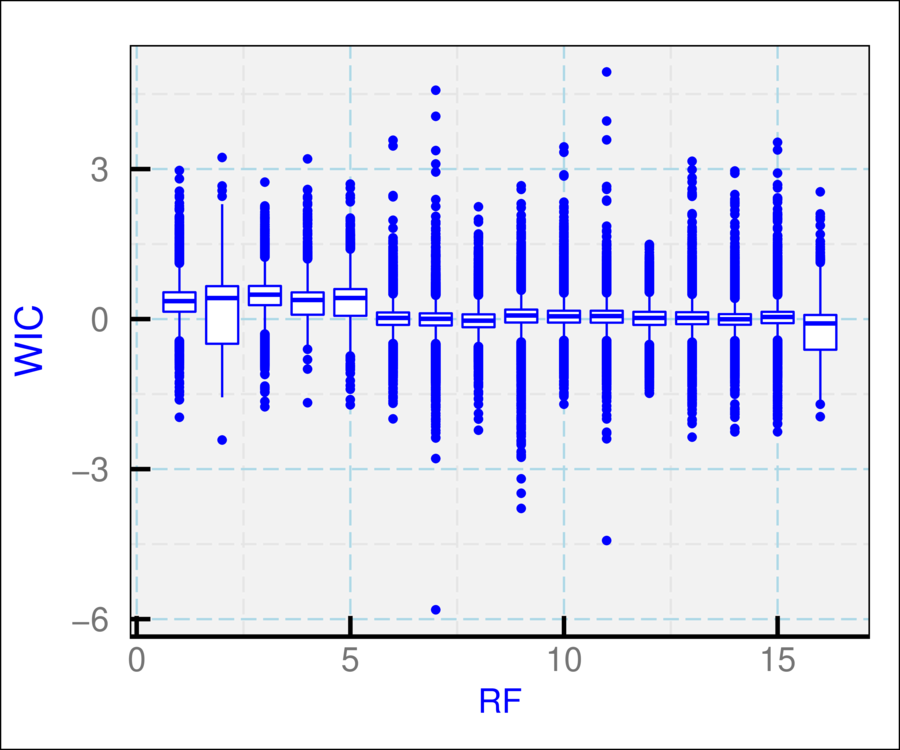
\includegraphics[width=\maxwidth]{figure/multiFlt-1} 

}

\caption[Distribution of values of the vertical wind for each research flight number]{Distribution of values of the vertical wind for each research flight number.}\label{fig:multiFlt}
\end{figure}


\end{knitrout}

\pagebreak{}

\begin{knitrout}
\definecolor{shadecolor}{rgb}{0.969, 0.969, 0.969}\color{fgcolor}\begin{kframe}
\begin{alltt}
\hlstd{Data} \hlopt \hlstd{dplyr}\hlopt{::}\hlkwd{select}\hlstd{(ATX, GGALT, RF)} \hlopt \hlstd{dplyr}\hlopt{::}\hlkwd{filter}\hlstd{(RF} \hlopt{>=} \hlnum{3} \hlopt{&} \hlstd{RF} \hlopt{<=} \hlnum{6}\hlstd{)} \hlopt
  \hlkwd{Rmutate}\hlstd{(}\hlkwc{RF} \hlstd{=} \hlkwd{as.character}\hlstd{(RF))} \hlopt
  \hlkwd{ggplot}\hlstd{()} \hlopt{+} \hlkwd{geom_point}\hlstd{(}\hlkwd{aes}\hlstd{(ATX, GGALT,} \hlkwc{color}\hlstd{=RF))} \hlopt{+}
  \hlkwd{theme_WAC}\hlstd{()}
\end{alltt}
\end{kframe}\begin{figure}

{\centering 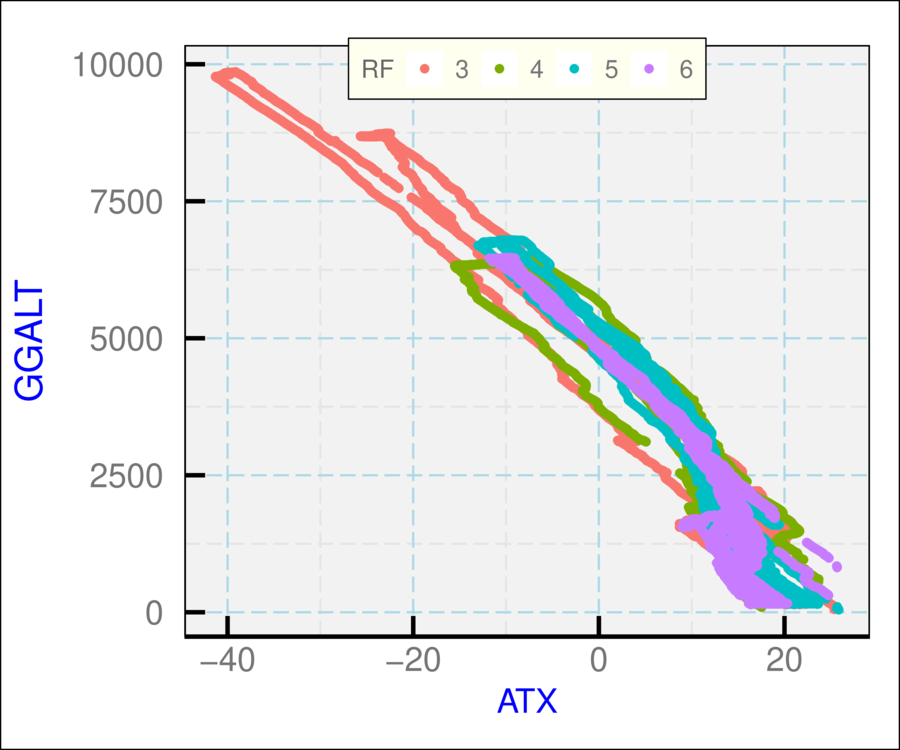
\includegraphics[width=\maxwidth]{figure/MF2-1} 

}

\caption[Measurements of temperature vs]{Measurements of temperature vs. altitude during research flights 3 to 6.}\label{fig:MF2}
\end{figure}


\end{knitrout}

\pagebreak{}

\begin{knitrout}
\definecolor{shadecolor}{rgb}{0.969, 0.969, 0.969}\color{fgcolor}\begin{kframe}
\begin{alltt}
\hlstd{Data} \hlopt \hlstd{dplyr}\hlopt{::}\hlkwd{select}\hlstd{(WIC, GGALT, RF)} \hlopt
         \hlstd{dplyr}\hlopt{::}\hlkwd{filter}\hlstd{(RF} \hlopt{==} \hlnum{4} \hlopt{|} \hlstd{RF} \hlopt{==} \hlnum{5}\hlstd{)} \hlopt
         \hlkwd{Rmutate}\hlstd{(}\hlkwc{RF} \hlstd{=} \hlkwd{sprintf}\hlstd{(}\hlstr{'research flight %d'}\hlstd{, RF))} \hlopt
         \hlkwd{ggplot}\hlstd{()} \hlopt{+} \hlkwd{geom_point}\hlstd{(}\hlkwd{aes}\hlstd{(WIC, GGALT))} \hlopt{+}
         \hlkwd{facet_wrap}\hlstd{(}\hlopt{~} \hlstd{RF,} \hlkwc{nrow}\hlstd{=}\hlnum{1}\hlstd{)} \hlopt{+} \hlcom{## see also facet_grid()}
         \hlkwd{theme_WAC}\hlstd{()}
\end{alltt}
\end{kframe}\begin{figure}

{\centering 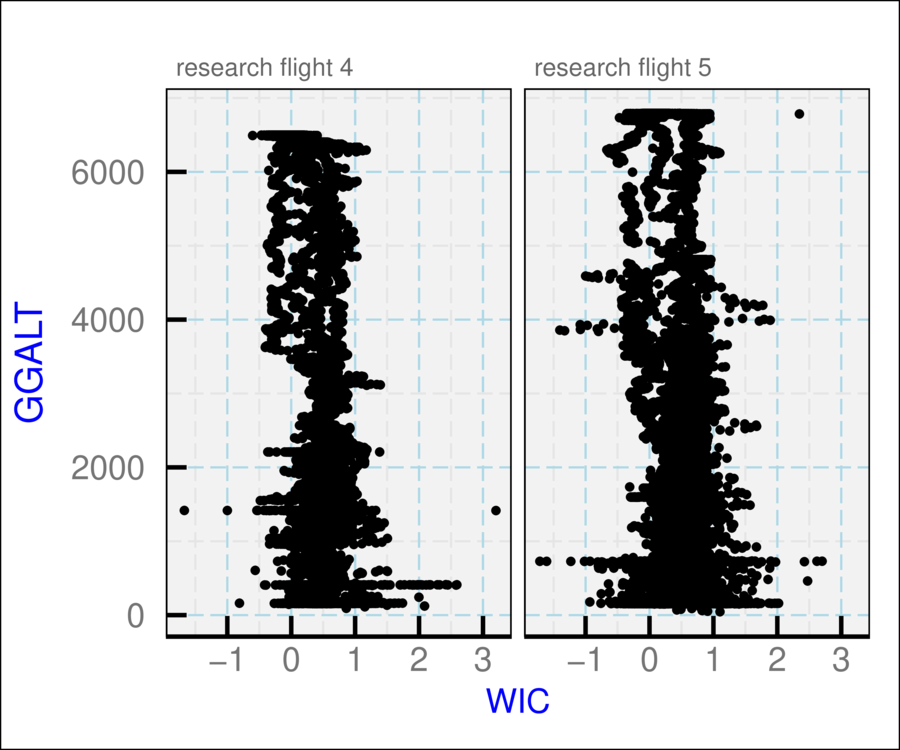
\includegraphics[width=\maxwidth]{figure/MF3-1} 

}

\caption[Example that uses faceted plots to show results from different research flights]{Example that uses faceted plots to show results from different research flights.}\label{fig:MF3}
\end{figure}


\end{knitrout}

\pagebreak{}

\begin{knitrout}
\definecolor{shadecolor}{rgb}{0.969, 0.969, 0.969}\color{fgcolor}\begin{kframe}
\begin{alltt}
\hlstd{Data} \hlopt \hlstd{dplyr}\hlopt{::}\hlkwd{select}\hlstd{(EWX, ATX, GGALT, RF)} \hlopt
         \hlstd{dplyr}\hlopt{::}\hlkwd{filter}\hlstd{(RF} \hlopt{==} \hlnum{4} \hlopt{|} \hlstd{RF} \hlopt{==} \hlnum{5}\hlstd{)} \hlopt
         \hlkwd{Rmutate}\hlstd{(}\hlkwc{RF} \hlstd{=} \hlkwd{sprintf}\hlstd{(}\hlstr{'research flight %d'}\hlstd{, RF))} \hlopt
         \hlkwd{Rmutate}\hlstd{(}\hlkwc{RH} \hlstd{=} \hlnum{100} \hlopt{*} \hlstd{EWX} \hlopt{/} \hlkwd{MurphyKoop}\hlstd{(ATX))} \hlopt  \hlcom{## new variable}
         \hlkwd{ggplot}\hlstd{()} \hlopt{+} \hlkwd{geom_path}\hlstd{(}\hlkwd{aes}\hlstd{(RH, GGALT,} \hlkwc{color}\hlstd{=RF))} \hlopt{+}
         \hlkwd{ylim}\hlstd{(}\hlkwd{c}\hlstd{(}\hlnum{0}\hlstd{,} \hlnum{7500}\hlstd{))} \hlopt{+}
         \hlkwd{xlab}\hlstd{(}\hlstr{'relative humidity [%]'}\hlstd{)} \hlopt{+}
         \hlkwd{ylab}\hlstd{(}\hlstr{'geometric altitude [m]'}\hlstd{)} \hlopt{+}
         \hlkwd{theme_WAC}\hlstd{()}
\end{alltt}
\end{kframe}\begin{figure}

{\centering 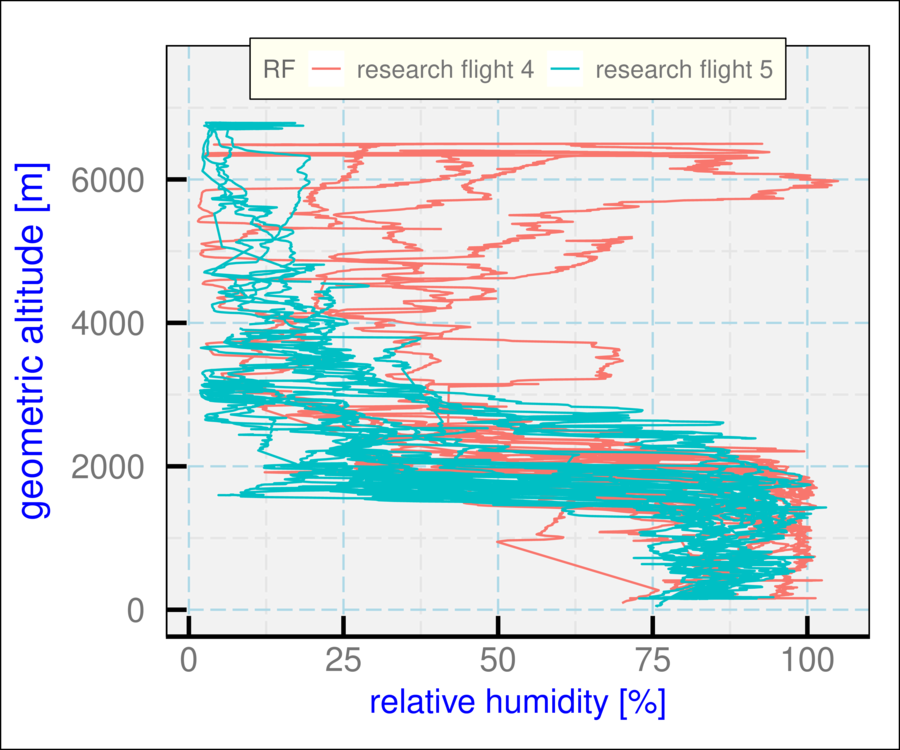
\includegraphics[width=\maxwidth]{figure/MF4-1} 

}

\caption[Example that uses faceted plots to show results from different research flights]{Example that uses faceted plots to show results from different research flights.}\label{fig:MF4}
\end{figure}


\end{knitrout}

\pagebreak{}

\begin{knitrout}
\definecolor{shadecolor}{rgb}{0.969, 0.969, 0.969}\color{fgcolor}\begin{kframe}
\begin{alltt}
\hlstd{Data} \hlopt \hlstd{dplyr}\hlopt{::}\hlkwd{group_by}\hlstd{(RF)} \hlopt \hlkwd{summarise}\hlstd{(}\hlkwc{mean} \hlstd{=} \hlkwd{mean}\hlstd{(WIC,} \hlkwc{na.rm}\hlstd{=}\hlnum{TRUE}\hlstd{))}
\end{alltt}
\begin{verbatim}
## # A tibble: 16 x 2
##       RF      mean
##    <dbl>     <dbl>
##  1     1  0.353   
##  2     2  0.142   
##  3     3  0.452   
##  4     4  0.328   
##  5     5  0.362   
##  6     6 -0.000691
##  7     7 -0.0391  
##  8     8 -0.0322  
##  9     9  0.0523  
## 10    10  0.0434  
## 11    11  0.0410  
## 12    12  0.00624 
## 13    13  0.0159  
## 14    14 -0.00931 
## 15    15  0.0351  
## 16    16 -0.228
\end{verbatim}
\end{kframe}
\end{knitrout}

\section{Comments re ``tibbles''}

The data.frames used by convention in Ranadu are inconsistent with
the ``tidy'' structure discussed in ``R for Data Analysis'' by
H.~Wickham because, for size-distribution variables such as those
produced by the CDP or UHSAS, the column consists of a two-dimensional
vector where the first dimension is the row and the second is the
concentration or count of particles in each bin. Data.frames not containing
such variables are ``tidy'' and can be converted to tibbles using
the function as\_tibble(). This will fail, however, for data.frames
that contain size-distribution variables. The function Ranadu::df2tibble()
will convert such data.frames to tibbles by converting the two-dimensional
vectors into lists. However, then the tibbles won't work with functions
like Ranadu::plotSD().\footnote{df2tibble() will also convert back to normal Ranadu structure with
the argument ``reverse = TRUE''.} Otherwise, the resulting tibbles are consistent with the Ranadu functions
including plotting and algorithm calculations.

\section{Reproducible research}

With the tools now available, it is possible to document analysis
projects to a degree that others can duplicate them using archived
information. Steps toward that goal are the topic of this section.
It is suggested that proper documentation of a project should include
these components:
\begin{enumerate}
\item The project report, documenting the analysis steps, data used, results
and interpretation.
\item Any code used.
\item Enough information on the underlying programming language (version
number, operating system, etc.) that someone else can use the same
code interpreter if necessary.
\item Locations of data files used, if in maintained archives, or copies
of the data sufficient to reproduce the results.
\item A discussion of the workflow required to reproduce the research. This
may include discussion of aspects of the code that may not be evident
to an inexperienced reader, documentation of investigations not included
in the report, reasons for choices made, and other advice to a person
seeking to reproduce the research that might not be appropriate in
the project report. The workflow document can be less formal and more
wordy or chatty that the project report if that material might be
useful to another analyst.
\end{enumerate}
Often, analysis steps are stutter-steps producing scattered material
that is hard to assemble, with different steps used to generate plots,
manipulate data, perform fits, construct derived data, combine multiple
and supplementary data sets, etc. Reproducibility does not mean necessarily
following that original path, but a logical path using the successful
steps should be documented. Essential but not adequate steps toward
reproducibility include making the code available in some repository
and ensuring that the data as used is archived where it is accessible.
The project report should indicate where these components of the analysis
are saved. The additional component that will usually be needed by
a reproducing analyst is a workflow document, which can be thought
of as guidance to a person wishing to verify or extend the results.

R tools are available that are of great utility in performing reproducible
research. The ``knitr'' package (see references) makes it possible
to assemble the text and code in the same file and to use knitr functions
to reference results from the code in the text or embed graphics in
the document as generated in the code. The ``Rnw'' format or other
alternative formats support this approach, and running that program
can generate the project report while running the specified code.
This avoids ad hoc assembly of figures, tables, and text from different
sources, which often obscures efforts to reproduce the work. A suggested
documentation package can then include the Rnw-format (or equivalent)
file, the report in text form, links to archives where the data are
available or alternately inclusion of the data in the archived project
package, a workflow discussion, and documentation of the version of
various programs and computer systems used. Some more information
on using knitr is included in the ``RSessions'' shinyApp tutorial,
in the ``reproducibility'' tab.

\section{The Ranadu Shiny app}

A shiny app that uses the Ranadu package to examine data files is
documented \href{https://drive.google.com/open?id=0B1kIUH45ca5AV1VDS1VxVDJaMmM}{here}.

%\attach{attachment}

%\attachm{first\\second}

%\cc{first attachment\\second\\3rd att}


\end{document}
